\DontNumberThisInToc
\DontFrameThisInToc
\glsresetall
\ChapterNumberCitation{La sélection active et motivée de l'action: un modèle des ganglions de la base}{The simple idea that planning is only experience read backward and combined by selection in suitable or successful combinations takes the mystery out of Nature and out of men's minds.}{William King Gregory}{10cm}
\section{Introduction}

Les noyaux gris centraux appelés encore les ganglions de la base [\gls{bg}] sont un ensemble de noyaux sous-corticaux inter-connectés qui font depuis longtemps l'objet d'études neuro-atomiques. Ces amas de cellules nerveuses reçoivent des projections de plusieurs régions du cortex cérébral (et d'autres régions extra-corticales) et renvoient des projections vers le cortex moteur, le cortex pré-moteur, l'aire motrice supplémentaire et d'autres aires frontales via le thalamus. Les ganglions de la base ont longtemps été considérés comme étant principalement impliqués dans la programmation et le contrôle des mouvements volontaires. Plusieurs cas cliniques neurologiques montrent que des lésions des noyaux gris centraux chez de nombreux patients sont accompagnés par des anomalies de mouvements. Différentes techniques récentes ont contribué à mieux comprendre l'organisation et le fonctionnement de ces noyaux. Ces techniques comprennent des études neuro-anatomiques des animaux et d'autopsie humaine, des enregistrements cellulaires provenant d'animaux et des humains qui subissent une chirurgie invasive du cerveau, des radiotraceurs, des études d'imagerie fonctionnelle, et des études comportementales des patients atteints de troubles moteurs, en particulier la maladie de Parkinson (PD, \textit{Parkinson Disease}) \cite{Ehringer:1960}, la maladie de Huntington \cite{Reiner:1988, Sapp:1995}, le syndrome de Tourette, etc. Ces ganglions sont également impliqués dans des fonctions plus cognitives, comme le traitement des émotions, de la mémoire et des comportements non moteurs. Plus généralement, de nombreuses études suggèrent que les \gls{bg} participent à la régulation de l'activité corticale par désinhibition (retrait de l'inhibition) du thalamus considéré comme relais, ce qui leur permet d'avoir un rôle primordial dans la \textit{sélection} des mouvements en assurant un ensemble d'intégrations dans des canaux distincts fonctionnellement \cite{Haber:2003}. En étudiant cette structure, nous examinerons la problématique concernant la manière d'assurer une prise de décision, à large échelle, lorsque des boucles différentes et des flux hétérogènes interagissent et servent à biaiser le traitement intrinsèque déterministe.\\

C'est dans le cadre de l'approche énactive, que nous avons choisi d'étudier la fonction de sélection des mouvements dans le circuit moteur des ganglions de la base décrit dans la suite. En effet, un modèle énactif en interaction active avec son environnement doit être capable de créer dynamiquement des représentations internes du contexte (perception active) et de choisir les mouvements adéquats même s'ils ne correspondent pas aux habitudes acquises ou aux réponses réflexes (sélection active).\\ 

La sélection des mouvements se place dans le cadre d'un problème plus général: la sélection de l'action [\gls{as}] étudiée dans plusieurs domaines. Ce problème implique de résoudre les conflits entre des comportements alternatifs concurrents dans un contexte donné. On distingue deux niveaux de concurrence, dont le niveau basique qui consiste à faire le choix entre des actions de la même famille pour atteindre un but commun. Par exemple, on propose à un sujet à jeun de choisir entre une pomme et une banane. Prendre l'une ou l'autre répondra au besoin de la faim. C'est le cas aussi de la sélection entre les cibles visuelles traitées dans le chapitre précédent. Par contre, proposer de choisir entre manger une pomme et boire un verre d'eau met en conflit deux besoins différents et par la suite un conflit d'accès à des ressources communes motrices ou cognitives. Ce dernier niveau est plus difficile à traiter et suggère de passer par la notion de \textit{saillance}. Il s'agit d'attribuer une valeur d'utilité ponctuelle dans le temps (un scalaire par exemple) à chacune des actions candidates permettant ainsi de les comparer et les classer par degré d'importance. Cette valeur devrait intuitivement dépendre du contexte sensoriel (perception), émotif (motivation) et temporel (mémoire).\\

Plusieurs modèles de la \gls{as} proposés dans la littérature sont plutôt conceptuels \cite{Brooks:1991, Rosenblatt:1995, It:1995} ne détaillant pas la mise en oeuvre algorithmique. D'autres modèles, pour estimer la valeur de la saillance, utilisent des sommes pondérées de plusieurs données ou des formules avec un réglage complexe de paramètres qui fait croire qu'il s'agit d'un estimateur réel \cite{Tyrrell:1993}. Enfin, des modèles d'apprentissage par renforcement (RL, \textit{reinforcement learning}) attribuent automatiquement des valeurs aux actions en fonction de la récompense obtenue qui reflète un jugement de l'action effectuée, donc une sorte d'évaluation en aval. La boucle principale des ganglions de la base (cortex-striatum-pallidum-thalamus-cortex, détaillée dans la suite) est souvent considérée comme \textit{acteur} dans une architecture \textit{acteur-critique} assurant une fonction de sélection de l'action. Son rôle principal est assimilé alors à un \textit{winner-takes-all} (faire gagner le plus fort) détaillé biologiquement. Il ne s'agit pas vraiment d'un choix de l'action, puisque le résultat de la sélection est déterminé à l'avance par le niveau de saillance donné en entrée, cette sélection peut être donc qualifiée de \textit{passive}.\\ 

Nous proposons dans ce chapitre un modèle de l'\gls{as} des \gls{bg} inspiré de données biologiques et des modèles de sélection de l'action de \cite{Gurney:2001a,Girard:2008} en mettant en œuvre une sélection que nous qualifierons d'\textit{active}. Une première section sera consacrée à décrire le fonctionnement des ganglions de la base tel qu'il est reporté dans la littérature en partant de la biologie pour arriver à la modélisation. Une deuxième section portera sur les hypothèses de notre modèle et sa position par rapport à \cite{Gurney:2001a,Gurney:2001b,Girard:2005a,Girard:2008}. Enfin les résultats seront présentés et discutés.\\

\section{Le fonctionnement des ganglions de la base}

Plusieurs études ont été consacrées à la structure et à la physiologie des \gls{bg} \cite{Houk:1994, Graybiel:1998, DeLong:2000}. Les \gls{bg} ont classiquement été décrits comme un ensemble d'une structure d'entrée (\textit{le striatum}) qui reçoit des projections directes de presque toutes les aires du cortex cérébral (sauf les aires primaires visuelle et auditive) \cite{Cherubini:1988,Kemp:1970,kitai:1976,McGeer:1977}, de deux structures de sortie (\textit{le palladum interne et la substance noire réticulée}) qui projettent vers le cortex (et des structures sous-corticales) via le thalamus et deux structures intrinsèques intermédiaires (\textit{le noyau sous-thalamique et le pallidum externe}) (fig \ref{fig:BG1}).\\

\begin{figure}
  \begin{center}
    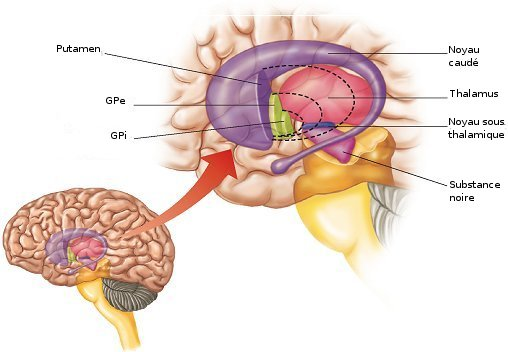
\includegraphics[width=0.6\textwidth]{figures/ch4_1_BG1}
  \end{center}
  \caption {Les différents noyaux des ganglions de la base. Le striatum (STR) composé du noyau caudé et du putamen. Le pallidum composé du segment interne (GPi) et segment externe (GPe). La substance noire composée de la partie compacte (SNc) et la partie réticulée (SNr). Le noyau sous thalamique (STN).} %Chevalier:1990,Deniau,}
  \label{fig:BG1}
\end{figure}


Ainsi, une caractéristique majeure de l'anatomie de \gls{bg} est leur implication dans plusieurs boucles avec le cortex cérébral (fig \ref{circuits}), appelées \textit{circuits cortico-basalo-thalamo-corticaux} \cite{Alexander:1986, Alexander:1990, Strick:1995}. Nous allons d'abord décrire les différents noyaux, ensuite, nous examinerons les différentes boucles.\\

\subsection {Anatomie}

\subsubsection{Le striatum}

Le striatum [\gls{str}] est le plus grand des noyaux gris centraux (à peu près $10^6$ neurones chacun connecté à $10^3$ synapses corticales). Il est composé du noyau caudé, du putamen et d'une partie différenciée connue sous le terme \textit{striatum ventral}\footnote{Le striatum ventral est particulièrement impliqué dans la régulation des comportements motivés comme les processus naturels liés à l'obtention d'une récompense ou les processus pathologiques de l'addiction. %(Ikemoto and Panksepp, 1996; Koob, 1992; Koob and Bloom, 1988; Robbins et al., 1989; Robledo and Koob, 1993; Robledo et al., 1992; Salamone, 1994
} qui englobe le noyau accumbens septi [\gls{nacc}], les parties ventromédiales du noyau caudé et du putamen et les cellules striatales des bulbes olfactives.\\

Le \gls{str} reçoit en effet de multiples afférences excitatrices glutamatergiques\footnote{Le glutamate, forme ionisée de l'acide glutamique, est le neurotransmetteur excitateur le plus important du système nerveux central.} qui proviennent globalement de toutes les aires du cortex cérébral sauf l'aire visuelle primaire V1 et l'aire auditive primaire [\gls{a1}] \cite{Albin:1995, Gerfen:1990, Kemp:1970, Cherubini:1988}. Le \gls{str} reçoit des entrées corticales liées aux paramètres des comportements \cite{Bauswein:1989,Turner:2000,Crutcher:1990}, liées au contexte \cite{Kimura:1990,Kimura:1992} et d'autres liées à la récompense \cite{Kawagoe:1998}. En outre du cortex, il reçoit des projections excitatrices des structures sous-corticales: thalamus [\gls{th}], hippocampe et amygdale \cite{Lapper:1992, Sadikot:1992}.\\ 

Au niveau microstructural, le \gls{str} peut être divisé en deux compartiments, le compartiment des \textit{striosomes} et celui des \textit{matrisomes} dont les connexions anatomiques sont distinctes\footnote{cette distinction entre matrisomes (matrices) et striosomes est encore un sujet de controverse et de même pour la distinction entre les récepteurs D1 et D2 décrits dans la suite}. Les connexions afférentes aux striosomes sont principalement issues du cortex orbital et des
régions limbiques (cingulaires et amygdaliennes). Le compartiment des matrices est innervé par les régions associatives (temporales, pariétales et préfrontales) et sensorimotrices du cortex. La voie striatonigrale décrite plus loin dans le texte réunit les neurones efférents des striosomes et se projette sur la substance noire compacte.\\

Plus généralement, le \gls{str} est constitué principalement de neurones épineux moyens [\gls{msn}] GABAergiques\footnote{L'acide $\gamma$-aminobutyrique, abrégé en GABA, est le principal neurotransmetteur inhibiteur du système nerveux central chez les mammifères et les oiseaux.} ($>90\%$). Au repos, ces neurones ont peu d'activité spontanée. Ils sont maintenus dans un état de faible excitabilité et sont peu réactifs aux influx corticaux excitateurs \cite{Nisenbaum:1995}. En conséquence, une forte activité synchronisée des projections cortico-striatales est nécessaire pour que les neurones de projection du striatum dépassent le seuil d'activation \cite {Mahon:2001, Mahon:2003}.\\

Ces neurones projettent d'une part sur le segment interne du pallidum [\gls{gpi}] et la substance noire réticulée [\gls{snr}]. D'autre part, ils projettent sur le noyau sous-thalamique [\gls{stn}] à travers le segment externe du pallidum [\gls{gpe}]. Les neurones qui projettent vers un noyau ou un autre sont morphologiquement indifférenciables et topographiquement mélangés  \cite {Feger:1984, Gerfen:1988, Parent:1989}. Ils commencent à décharger avant que le mouvement ne commence. Ceci suggère que le striatum participe à la programmation du mouvement volontaire. \cite{Lidsky:1985} ont signalé une activité neuronale striatale qui semblait être liée uniquement à des mouvements ou des stimuli sensoriels qui se produisent dans un contexte particulier. En effet, le \gls{str} participe à filtrer les informations corticales les plus pertinentes et transformer les signaux corticaux selon le contexte afin d'inhiber localement les noyaux de sorties des \gls{bg}. Il est principalement impliqué dans l'apprentissage de compétences motrices, perceptives et cognitives\cite{Joel:1994, Suzuki:2001}. \\

\subsubsection{Le pallidum externe}

Le segment externe du pallidum est une structure intermédiaire qui reçoit des projections inhibitrices du \gls{str} et d'autres excitatrices du \gls{stn} et renvoie des projections GABAergiques inhibitrices vers le \gls{str} et le \gls{gpi} mais majoritairement vers le \gls{stn} \cite{Rouzaire:1980}. Il semble agir en opposition aux projections striatales \cite{Alexander:1990}.\\


\subsubsection{Le pallidum interne et la substance noire réticulée}

Ces deux noyaux composés de neurones similaires sont considérés comme une seule structure fonctionnelle de sortie \cite {Carpenter:1981}. Ils sont toniquement actifs, i.e déchargent au repos à des taux élevés en l'absence de l'entrée striatale leur imposant une pause ou une réduction de leur cadence de décharge. L'effet net de l'entrée du striatum au \gls{gpi}/\gls{snr} est une réduction de l'inhibition tonique exercée par les cellules pallidales sur leurs cibles (désinhibition) permettant donc une augmentation du taux de décharge dans les cellules correspondantes (thalamus, colliculus supérieur...). Donc leur désinhibition permet en particulier d'activer les aires motrices via le thalamus par excitations glutamatergiques des aires corticales frontales et d'initier ainsi les mouvements moteurs bloqués toniquement \cite{Nauta:1966}.\\


\subsubsection{Le noyau sous-thalamique}

Le noyau sous-thalamique est le seul noyau excitateur des \gls{bg}, il re\c coit des projections inhibitrices du \gls{gpe} et ses neurones glutaminergiques renvoient des projections excitatrices répandues\footnote{efférences divergentes: chaque axone du \gls{stn} innerve de nombreux neurones du \gls{gpi}} (diffuses) au \gls{gpi} et à la \gls{snr} \cite{Parent:1993} permettant ainsi d'inhiber les générateurs de motifs moteurs [\glspl{mpg}] des mouvements concurrents. Il reçoit aussi des afférences excitatrices principalement des aires motrices du lobe frontal \cite{Monakow:1978,Kitai:1981,Nambu:1996,Nambu:1997}. L'entrée corticale vers le \gls{stn} est principalement liée au mouvement \cite{Delong:1985,Wichmann:1994}.\\

\subsubsection{La substance noire compacte}

Alors que la \gls{snr} est composée de neurones GABAergiques, la \gls{snc} est composée plutôt de neurones dopaminergiques qui projettent principalement sur les \glspl{msn} dans le \gls{str}. On parle donc de la voie nigro-striatale \cite{Haber:2000}. Au niveau dorsomedian de la \gls{snr} se trouve l'aire tegmentale ventrale, compos\'ee de neurones dopaminergiques identiques à ceux de la \gls{snc}. Ces neurones sont qualifiés ainsi parce qu'ils produisent un neuro-modulateur appelé \textit{la dopamine} [\gls{da}]. Le rôle de la dopamine au sein des \gls{bg} est complexe et en grande partie non résolu. \\

\begin{figure}
  \begin{center}
    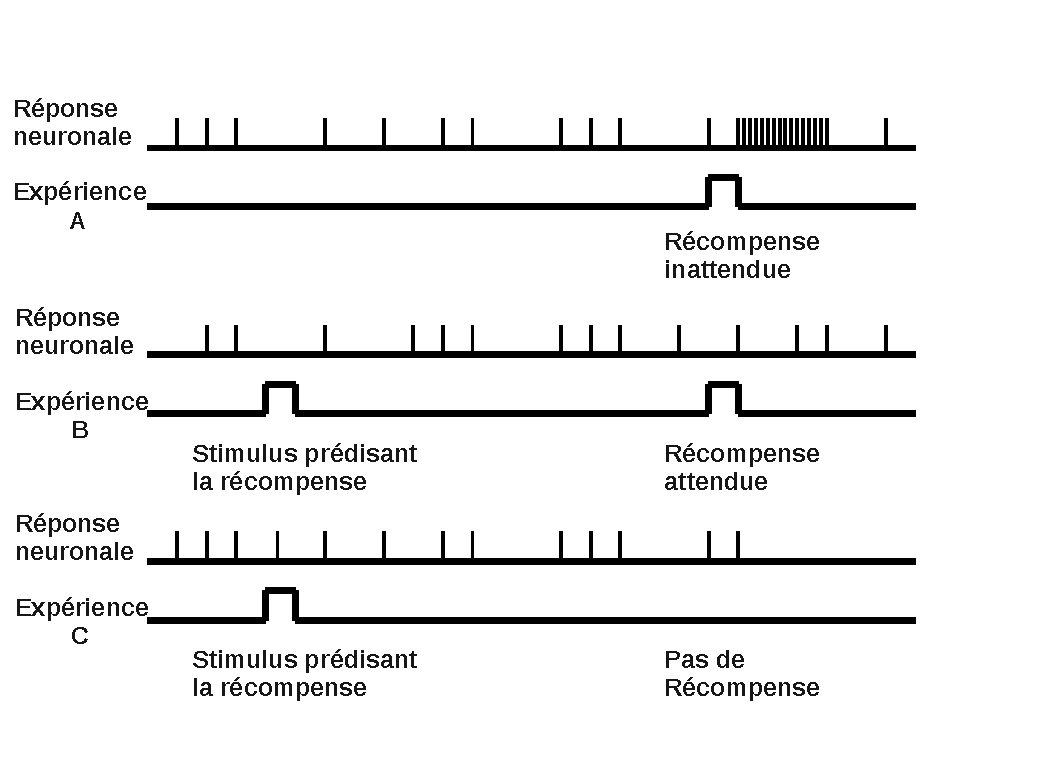
\includegraphics[width=0.65\textwidth]{figures/ch4_2_dopamine}
  \end{center}
  \caption { Les neurones dopaminergiques signalent une récompense inattendue ou une absence inattendue de récompense \protect\cite{Schultz:1997}. (A) Si une récompense arrive de manière inattendue, l'activité du neurone dopaminergique augmente. (B) Si une récompense arrive suite à un stimulus la prédisant appris par le singe, l'activation n'est pas modifiée, signalant ainsi que tout se déroule normalement. (C) Si suite à un stimulus prédisant la récompense, rien ne se produit (pas de récompense), la décharge neuronale est inhibée.}
  \label{dopamine}
\end{figure}

Globalement, la dopamine est impliquée dans deux fonctions fondamentales du cerveau: activation motrice et apprentissage par récompense des associations stimulus-réponse (S-R). Il s'agit de choisir une action en réponse à un contexte sensoriel donné. Son effet de base est d'agir sur l'activité du striatum en projetant sur les récepteurs dopaminergiques D1 et les récepteurs D2 des neurones striataux. En effet, la dopamine excite les récepteurs D1 et inhibe les récepteurs D2. Avec l'action de la dopamine, la réponse de ces neurones à une entrée corticale est modifiée de telle sorte que les profils de l'activité striatale qui se corrèlent avec l'exécution des tâches suivies de récompense sont renforcés par l'augmentation de la force (poids) synaptique des entrées corticales.\\

La dopamine a d'abord été considérée comme un signal de récompense. Plusieurs enregistrements électrophysiologiques, chez des singes apprenant des tâches comportementales, ont montré des neurones dopaminergiques qui déchargent de façon phasique quand une récompense inattendue arrive mais quand la même expérience est répétée plusieurs fois, la décharge se décale dans le temps pour répondre aux stimuli prédisant ainsi la récompense et ne plus coïncider donc avec la récompense. La dopamine est ainsi considérée comme un signal d'erreur de récompense (corrélée donc avec l'anticipation de la récompense) et non plus un signal de récompense \cite{Houk:1995, Schultz:1997, Hollerman:1998, Morris:2004, Takikawa:2004, Bayer:2005,Schultz:2006} (fig \ref{dopamine}). Mais une grande partie de l'activité de la \gls{snc} semble être tonique plutôt que phasique ou transitoire, ce qui rend difficile d'établir la contribution explicite de cette voie à la commande motrice.\\

%\cite{Doya 1999}La dopamine code pour le prediction de la récompense $DA(t)=r(t)+1/[(V(t+1)-V(t)]$ \cite{Schultz 1997}.
%La plasticité dépend de la dopamine \cite{wickebs:1995}

\subsection{Organisation en boucles fonctionnelles}

%L'entrée corticale vers \gls{bg} est organisée en bandes longitudinales de projections parallèles. 

Les \gls{bg} semblent fonctionner via un système de boucles parallèles initialement décrites comme cinq circuits dissociés et parallèles: un circuit moteur qui inclut les aires motrices, prémotrices et motrices supplémentaires, un circuit oculomoteur passant par les champs oculaires frontaux [\glspl{fef}], deux circuits préfrontaux passant respectivement par le cortex dorsolatéral préfrontal et orbitofrontal latéral et finalement un circuit limbique reliant le cortex cingulaire et orbitofrontal médian \cite{Alexander:1990, Alexander:1986, Albin:1989,Mink:1996}. Cette forme d'organisation est particulièrement adaptée pour des effets de rétroaction (\textit{feed-back}) et d'anticipation (\textit{feed-forward}). Ces boucles permettent de sélectionner des états corticaux, de les intégrer et de contrôler leur succession \cite{Berns:1998, Beiser:1998, Hikosaka:1999, Nakahara:2001} (fig \ref{circuits}).\\


\begin{figure}
  \begin{center}
    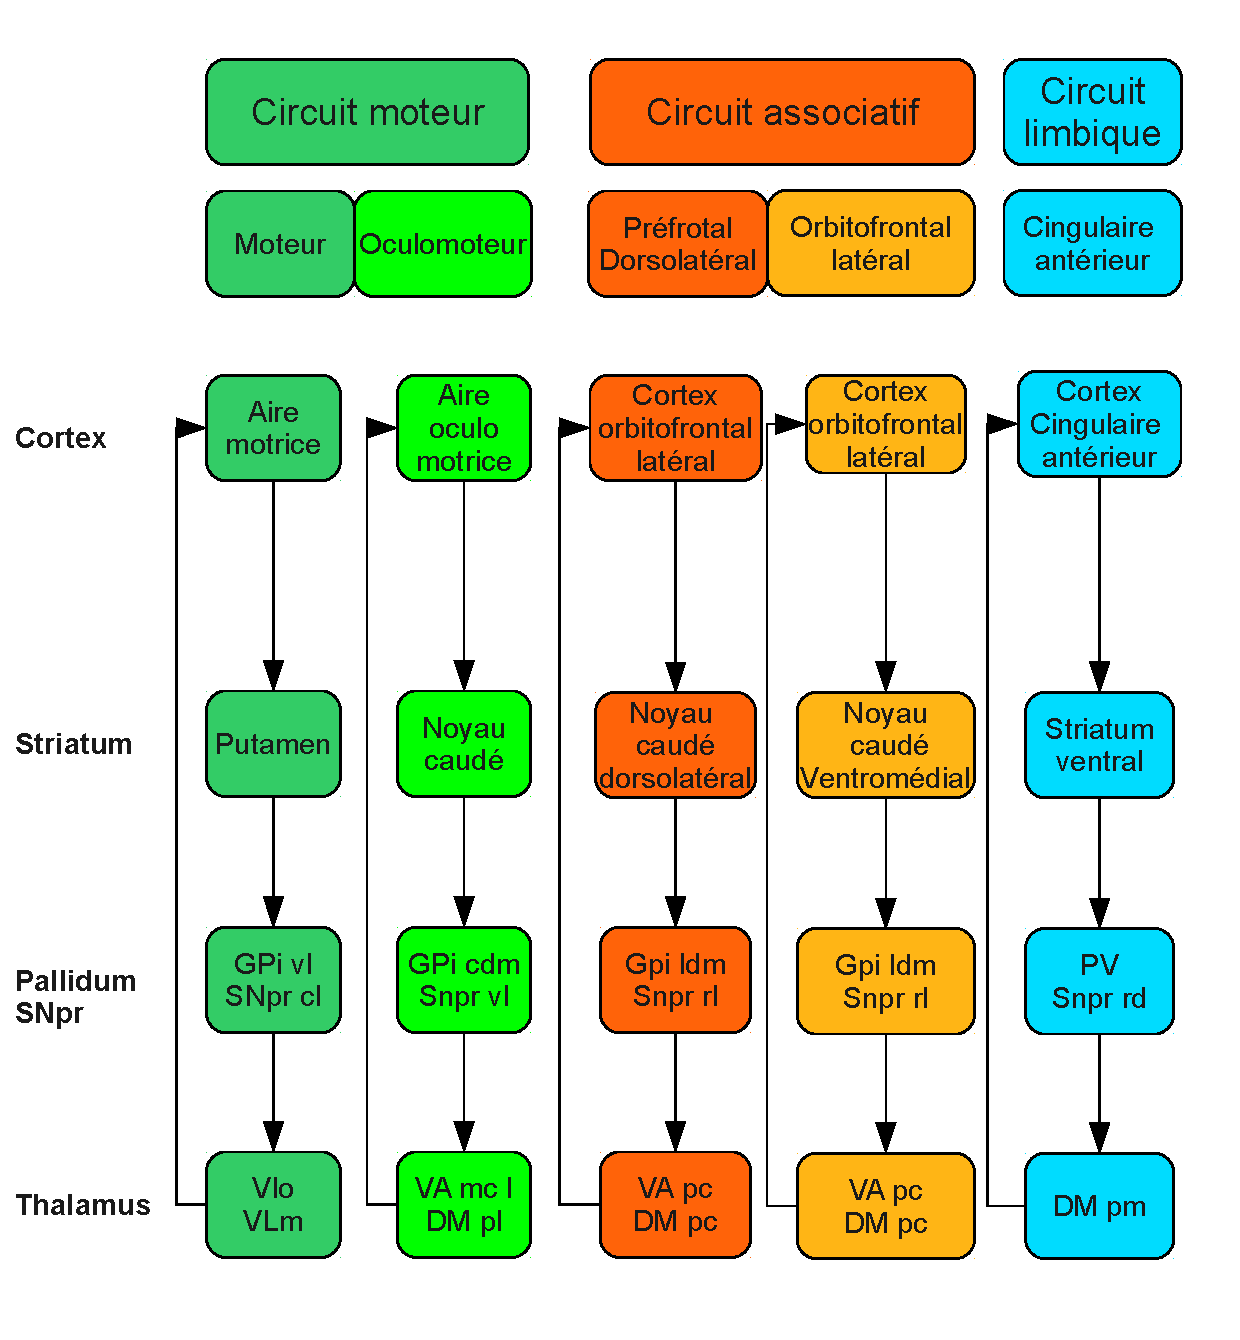
\includegraphics[width=14cm,height=10cm]{figures/ch4_3_circuits}
  \end{center}
  \caption {Les différents circuits cortico-basalo-thalamo-corticaux. SNpr: substance noire réticulée, GPi: pallidum interne, PV: pallidum ventral, VAmc: noyau ventral antérieur du thalamus, VL: noyau ventro-latéral du thalamus, DM: noyau dorso-médian du thalamus, mc: magnocellulaire, pc: parvocellulaire, pm: paralamellaire, cl: caudolatéral, cdm: caudal dorsomédian, dl: dorsolatéral, l: latéral, ldm: latéral dorso-médian, m: médian, mdm: médian dorso-médian, pl: postéro-latéral, pm: postéro-médian, rd: rostro-dorsal, rl: rostro-latéral, rm: rostro-médian, vl: ventrolatéral, vm: ventromédian. [Adapté de \protect\cite{Alexander:1986}]}
  \label{circuits}
\end{figure}


Par la suite, ces cinq circuits ont été regroupés dans un modèle à trois circuits fonctionnels et distincts où chacun des \gls{bg} possède un compartiment sensorimoteur, un compartiment associatif et un compartiment limbique \cite{Parent:1990, Parent:1993,Joel:1994}. Des travaux chez le singe ont démontré, par micro-injections d'agents pharmacologiques, des réponses comportementales et une connectivité anatomique différente selon que l'un ou l'autre des compartiments est stimulé \cite{Grabli:2004}. Les trois circuits présentent la même organisation globale, les structures intermédiaires diffèrent en fonction du type de l'information traitée. Cette description postule donc que chacune des boucles met en jeu des subdivisions différentes dans chacune des structures des \gls{bg}. \\ 

Même si ces descriptions insistent sur la séparation entre les différentes boucles, les interférences entre elles peuvent être cruciales pour les activités corrélées dans les différentes régions corticales. En effet, les patients parkinsoniens sont également altérés dans le traitement et l'utilisation des informations proprioceptives. En règle générale, ils ont du mal  à coordonner et intégrer les différentes composantes élémentaires du mouvement en vue d'aboutir à un mouvement composé volontaire performant \cite{Schettino:2006}. Si le sujet dans l'exemple précédent, choisit de prendre le verre d'eau, ceci active le cortex frontal qui à son tour projette sur le cortex moteur qui détermine sa trajectoire en fonction du retour du cortex visuel. Puis le mouvement est déclenché en coordonnant la séquence de muscles à activer au cours du mouvement.\\

Ceci suggère que les \gls{bg} facilitent la liaison entre les différentes régions corticales qui agissent de manière coordonnée pour façonner le comportement moteur et participent à la planification\footnote{la planification cognitive est l'une des fonctions exécutives qui comprend les processus neurologiques impliqués dans la formulation, l'évaluation et la sélection d'une séquence de pensées et d'actions pour atteindre un objectif souhaité.} des comportements moteurs pour l'exécution de tâches complexes \cite{Elsinger:2006, Wu:2005, Houk:1995}. La perturbation des circuits neuronaux, par l'intermédiaire de divers mécanismes tels que des lésions cérébrales traumatiques, ou les effets des maladies neuro-dégénératives entre cette région du cortex frontal et les ganglions de la base, spécifiquement le striatum (voie cortico-striatale), peuvent perturber les processus nécessaires à la planification \cite{Houk:1995} mais nous ne nous intéresserons pas à cette fonction et seules des tâches simples seront considérées. Nous passerons en revue les différentes fonctions des \gls{bg} proposées dans la littérature pour s'intéresser en particulier au circuit moteur et son rôle dans la sélection de l'action.\\

%%%%%%%%%%%%%%%%%%%%%%%%%%%%%%%%%%%%%%%%%%%%%%%%%%%%%%%%%%%%%%%%%%%%%%%%%%%%%%%%%%%%%%%%%%%%%%%%%%%%%%%%%%%%%%%%%%%%%%%%%%%%%%%%%%%%%%%%%%%%%%%%%%%%%%
\subsection{Fonctions des ganglions de la base}

Les ganglions de la base sont essentiellement connus pour leur rôle dans le contrôle moteur, mais leur fonction ne se limite pas au traitement de l'information sensorimotrice, ils participent également à diverses fonctions cognitives et comportementales \cite{Middleton:2000}.\\

\subsubsection{Fonctions motrices : architecture du circuit moteur}

Le circuit moteur des \gls{bg} est le mieux étudié. Il se base sur les projections des aires corticales frontales associatives, principalement les régions prémotrice et motrice supplémentaire et le cortex préfrontal dorsolatéral sur le striatum antérieur. Une fois l'information traitée dans les \gls{bg}, elle est transmise via le thalamus moteur vers le cortex préfrontal et prémoteur. Les \gls{bg} modulent à la fois le système moteur latéral ( mouvements volontaires) et le système moteur médian (posture et tonicité des muscles).\\

En effet, une grande partie de l'entrée des \gls{bg} arrive au niveau de striatum qui projette vers la sortie \gls{gpi}/\gls{snr} via deux chemins : la ``voie directe'' et la ``voie indirecte'', qui semblent avoir des effets contraires \cite{Albin:1989} (détaillés dans la section suivante). Au repos, le thalamus est inhibé par \gls{gpi}/\gls{snr}. L'inhibition de certains neurones peut être enlevée sélectivement via la voie directe: le striatum inhibe certains neurones de \gls{gpi}/\gls{snr}. La boucle qui relie le néocortex, le striatum, le palladium interne, le thalamus et le cortex frontal est classiquement considérée comme la boucle principale des ganglions de la base. Mais il s'y ajoute la projection en aval de la substance noire réticulée principalement vers le colliculus supérieur, participant ainsi au contrôle oculomoteur des saccades visuelles \cite{Graybiel:1978, Hikosaka:1983a, Hikosaka:1983b, Hikosaka:1983c}.\\

A cette boucle principale, s'ajoutent aussi des boucles latérales qui participent particulièrement à la régulation de l'activité du palladium, comme la voie indirecte qui module la sortie des \gls{bg} \cite{Percheron:1991}. Une fois stimulés par le cortex, les neurones du striatum dans les axones de la voie indirecte envoient des projections inhibitrices sur les cellules du pallidum externe, qui inhibe de manière tonique le noyau sous-thalamique. Cette inhibition (par le \gls{str}) des projections inhibitrices du \gls{gpe}, se traduit par une réduction nette de l'inhibition du \gls{stn}. Finalement le \gls{stn}, à son tour, envoie des projections excitatrices au complexe \gls{snr}/\gls{gpi} (qui inhibe toniquement le thalamus). Le résultat final est en particulier une inhibition du thalamus et, par conséquent, une diminution de la stimulation du cortex moteur par le thalamus et l'activité musculaire est réduite.\\

Cette distinction de voies est surtout étudiée dans le circuit moteur et elle se base sur les cibles des projections des neurones striataux et leur sensibilité à la dopamine. Il est classiquement considéré que la voie directe contient des récepteurs D1 et la voie indirecte contient des récepteurs D2 \cite{Ince:1997, Gerfen:1995, Bloch:1994, Gerfen:1994} mais certaines études favorisent l'existence des deux types de récepteurs dans les deux voies \cite{Aizman:2000,Surmeier:1996}. Comme introduit dans \cite{Frank:2005}, on distingue donc deux types de signaux : le \textit{``GO signal''} qui sélectionne l'action adéquate à exécuter en réponse à un stimulus et le \textit{ ``NO-GO signal''} qui au contraire supprime une réponse. Cette distinction est fondée sur les activations neuronales qui ont été remarquées dans le striatum chez le singe en réponse à deux stimuli (clés) qui indiquent si le singe doit exécuter (GO) ou supprimer (NO-GO) un mouvement du bras \cite{Apicella:1992}. L'augmentation de la dopamine cause une augmentation du contraste entre les deux chemins et par conséquent sur les niveaux des signaux GO/NO-GO servant plus tard à diriger un apprentissage synaptique.\\

En considérant en plus l'entrée corticale vers le noyau sous-thalamique \cite{Mink:1993,Kita:1994, Mink:1996, Nambu:2000}, à ces deux voies s'ajoute la \textit{``voie hyperdirecte''} \cite{Nambu:2002, Joel:1997, Gerfen:2000}. Une stimulation corticale induit une excitation à courte latence, suivie par une inhibition puis une excitation retardée dans les neurones pallidaux de singes. L'excitation précoce est considérée comme provenant de la voie cortico-\gls{stn}-pallidiale (hyperdirecte) comme argumenté dans \cite{Nambu:2000}. Cette voie s'avère être une voie excitatrice rapide par opposition à celles qui passent par le striatum et qui semblent être plus lentes. Le modèle de Nambu qui introduit cette voie propose de considérer que lorsqu'un mouvement volontaire est présenté au niveau cortical, un premier message via la voie hyperdirecte excite de manière diffuse la \gls{snr}/le \gls{gpi} et par conséquent inhibe le thalamus et ses projections corticales. Cette inhibition est globale (non locale), il s'agit d'un signal de réinitialisation,\textit{``RESET''}. L'effet résultant est un effet {\em center-surround}: une sélection focalisée sur l'action adéquate avec une inhibition des commandes motrices compétitives \cite{Mink:1993, Mink:1996,Hikosaka:2000, Chevalier:1990, Hikosaka:1988}. \\

Des enregistrements de l'activité neuronale au niveau du \gls{gpi} montrent un comportement tri-phasique dont l'interprétation donne un éclairage sur le rôle des \gls{bg} dans l'initiation des mouvements. D'abord une augmentation de l'inhibition tonique juste après la stimulation du cortex somatomoteur (voie rapide hyperdirecte), suivie d'une baisse d'activité (voie directe) pour finir à nouveau par une hausse d'activité (voie lente indirecte) au niveau d'un neurone du \gls{gpi} \cite{Nambu:2008}.\\

Ces différentes voies agissent donc comme une balance réglable qui contrôle finement le niveau d'activation de la sortie des noyaux gris centraux. Un bon équilibre est nécessaire pour un fonctionnement moteur normal. En effet, l'activation sélective des différents éléments de ces voies détermine les activités spécifiques qui vont s'exprimer tandis que les autres sont fortement inhibées. Il en résulte deux types de sélection par compétition entre les voies \cite{Hikosaka:1993}. D'une part, une compétition simultanée: une inhibition globale via les voies indirecte et hyperdirecte contre une désinhibition sélective via la voie directe. D'autre part, une compétition séquentielle due aux différences entre les constantes temporelles des différentes projections. Plus généralement, pour générer un mouvement, il n'est pas suffisant d'activer le \gls{mpg} responsable de l'action souhaitée à cause de la présence de \glspl{mpg} concurrents qui sont préalablement activés et doivent se désactiver \cite{O:2006,Redgrave:1999}. Donc la première fonction motrice des \gls{bg} consiste à sélectionner le mouvement à effectuer en désinhibant le thalamus d'une part et supprimer toutes les autres actions concurrentes d'une autre part. \\

Rappelons que les structures de sortie de \gls{bg} projettent aussi sur le colliculus supérieur (qui à son tour projette sur le thalamus), donc inhibent de manière similaire les mouvements des yeux. D'après les études de saccades chez les singes, l'activité tonique des neurones de la \gls{snr} inhibe les neurones colliculaires qui contrôlent les saccades oculaires. Lorsque les neurones striataux de la voie directe sont excités par les champs oculaires frontaux, certains neurones de la \gls{snr} sont momentanément inhibés libérant ainsi les neurones colliculaires appropriés pour signaler la cible du mouvement oculaire. Le singe déplace alors son regard vers un nouvel emplacement.\\ 

Plus généralement, les \gls{bg} assurent qu'un seul programme moteur, parmi les programmes primitifs possibles, soit actif à un moment donné en inhibant tout conflit et toute concurrence. Ce programme est libéré temporairement ce qui lui permet d'être exécuté par le corps. Ainsi, les \gls{bg} agissent comme un interrupteur qui permet l'exécution de programmes automatiques et sont considéré donc comme un substrat de sélection de l'action motrice\cite{Kropotov:1999,Mink:1996,Redgrave:1999, Prescott:2007,Gurney:2001a, Frank:2005}. \\

\subsubsection{Fonctions cognitives}

Comme mentionné précédemment, certains circuits impliquant les \gls{bg}, impliquent aussi le cortex associatif préfrontal et le cortex limbique. En plus de son rôle moteur, les \gls{bg} participent à plusieurs processus cognitifs et fonctions sensorielles (motivation, sélection, mémoire, apprentissage ...) \cite{Berns:1996,Redgrave:1999}. Certaines personnes atteintes de la maladie de Parkinson souffrent de déficits cognitifs tels que la suppression visuelle et les problèmes de reconnaissance des visages \cite{Jacobs:1995}. D'autres patients présentant des lésions du pallidum ou de la \gls{snr} ont des troubles de mémoire de travail, un comportement obsessionnel et des hallucinations visuelles \cite{Laplane:1989}. En particulier, l'implication des \gls{bg} dans la mémoire de travail peut être considérée comme une extension de son rôle dans la sélection de l'action \cite{Prescott:2003, Kawagoe:1998}. \\

En outre, les \gls{bg} semblent être impliqués dans certaines tâches d'apprentissage comme la mémorisation des associations stimuli/réponses \cite{Hikosaka:1998, Perez:2001}. Les patients Parkinsoniens n'arrivent pas à réussir de telles tâches \cite{Knowlton:1996}.  Des enregistrements de neurones striataux chez les singes ont montré que les propriétés de l'activation du striatum changent lorsqu'une association est construite entre un stimulus sensoriel spécifique et une réponse motrice appropriée \cite{Aosaki:1994}.\\


D'autres formes d'apprentissage semblent également être influencées par les \gls{bg}. Des études physiologiques ont montré que des parties du striatum et du pallidum sont activées pendant l'exécution des tâches qui nécessitent l'apprentissage d'une séquence de mouvements \cite{Kermadi:1995, Cromwell:1996,Berns:1998}. L'apprentissage de séquences nécessite soit la présence d'une mémoire de travail assurée par un feedback local par exemple \cite{Smith:1994}, soit un feedback de la sortie des \gls{bg} vers le cortex mais cette voie semble être très lente \cite{Alexander:1986,Hedreen:1991}. C'est ainsi qu'une revue datant de 2000, \cite{Gillies:2000} classe les modèles computationnels des \gls{bg} en 3 familles : Les modèles de traitement séquentiel \cite{Berns:1998}, les modèles de sélection de l'action \cite{Gurney:2001a} et les modèles d'apprentissage par renforcement comme les travaux de \cite{Schultz:2000a, Schultz:2000b} en particulier les modèles d'acteur-critique \cite{Barto:1995,Houk:1995,Brown:1999,Suri:2001,Suri:1998,Contreras:1999}.\\

Ces derniers modèles considèrent les \gls{bg} comme une architecture permettant de prédire et d'évaluer la récompense à chaque pas de l'épisode de la simulation \cite{Joel:2002,Niv:2001}. Le principe est de choisir grâce à la partie ``acteur'', à partir des états courants et des connaissances actuelles, la meilleure action à faire en se basant sur les prédictions de la partie ``critique''. L'architecture acteur-critique fait partie des méthodes à base de \textit{différence temporelle (TD)} \cite{Samuel:2000,Klopf:1972,Sutton:1988, Houk:1995,Joel:2002} qui servent à résoudre des problèmes de prédiction (étant donné l'état actuel des variables, quel avantage ou récompense peut on espérer gagner dans le futur). Les erreurs de prédictions permettent d'adapter et de corriger les deux agents \cite{Sutton:1998}. L'analogie entre les \gls{bg} et les modèles d'acteur-critique s'appuie sur la forte ressemblance entre les activités des neurones dopaminergiques (fig \ref{dopamine}) et le signal d'erreur de prédiction ainsi que le fait que la plasticité synaptique dépend à long terme de la dopamine \cite{Calabresi:2000,Wickens:1996}. En effet, La dopamine phasique (par opposition à la dopamine tonique) est supposée résulter de l'erreur dans le feedback moteur et servir à la modulation du seuil de facilitation ou de suppression des commandes motrices en réponse à un stimulus.\\
 
Certains modèles computationnels se concentrent sur le mécanisme d'apprentissage lui même sans s'intéresser à la structure du cerveau \cite{Perez:2001}. D'autres s'intéressent aux structures mais partiellement à l'apprentissage, soit à apprendre le signal d'erreur dopaminergique \cite{Brown:1999, Barto:1995}, soit à choisir des signaux d'erreur à la main pour apprendre des associations \cite{Frank:2005,Gurney:2001a,Berns:1998}. Par exemple, \cite{Frank:2005} propose un modèle qui apprend à choisir entre deux actions en réponse à un ensemble d'entrées. Les deux voies permettent d'apprendre les conditions du \textit{gating} (GO) et de la suppression (NO-GO). Ce modèle a été proposé comme une base théorique pour un apprentissage procédural des tâches cognitives. D'autres chercheurs se sont intéressés au codage de l'information de la récompense et à la sélection de la réponse dans la circuiterie biologique \cite{Brown:2004,Gurney:2001a,Beiser:1998} sans modéliser l'apprentissage implicite. Il en a résulté des modèles de critiques pour la prédiction et la simulation des effets de la dopamine \cite{Brown:2004} et des modèles d'acteurs détaillés pour des tâches de sélection avec une seule motivation \cite{Frank:2006,Khamassi:2004,Khamassi:2005} ou multimotivationnelles \cite{Dayan:2001,Girard:2008}.\\


Enfin, un rôle très peu étudié des \gls{bg} correspond à la {réduction de dimensionnalité} qui s'opère entre l'entrée des \gls{bg} et leur sortie basé sur des constatations anatomiques. Le nombre de neurones corticaux qui projettent sur le striatum est cent fois plus grand que le nombre de neurones striataux \cite{Kincaid:1998} avec une réduction supplémentaire identique au niveau du \gls{gpi} \cite{Percheron:1994}. Ensuite, on observe un élargissement en partant du \gls{gpi} vers le cortex en passant par le thalamus \cite{Arecchi:1996,Sidibe:1997}. Des études théoriques ont montré que les réseaux de neurones réalisent des réductions de dimensionnalités par règles hebbiennes \cite{Oja:1982} pour les connexions intercouches et règles anti-hebbiennes pour les connexions latérales intracouches \cite{Foldiak:1989}. L'idée est de considérer les \gls{bg} comme un commutateur adaptatif central qui ordonne les informations entrantes selon les priorités et les compresse pour activer le cortex frontal à travers un nombre limité de canaux. Deux stratégies sont proposées, réduire la dimensionnalité [PCA,(\textit{Principal Component Analysis})] ou bien réduire l'information (voir \cite{Bar:2003} pour plus de détails). \\


Nous allons nous intéresser en particulier au rôle des \gls{bg} dans la sélection de l'action en considérant donc principalement le circuit moteur. Nous allons décrire d'abord quelques modèles existants mettant en oeuvre la sélection intrinsèque par désinhibition basée sur l'interaction entre plusieurs voies concurrentes, dans les \gls{bg}, pour expliciter dans la suite notre proposition.\\ 
%-------------------------------------------------------------------

\subsection{ Modèles computationnels du circuit moteur}

\subsubsection{Le modèle classique}

Un des premiers modèles de ganglions de la base est celui de Albin-Delong \cite{Albin:1989, DeLong:1990}. Il a été inspiré des troubles de mouvements chez les patients parkinsoniens. En effet, dans la maladie de Parkinson, qui est un trouble hypo-kinétique \footnote{les patients hypo-kinétiques sont plus lents que la normale, prennent plus de temps pour accomplir certaines tâches, génèrent moins de force. Les patients parkinsoniens sont également hypo-métriques et font des mouvements à amplitudes plus faibles que la normale en essayant d'atteindre une cible}, l'hyperactivité relative de la voie indirecte conduit à l'excitation excessive du \gls{gpi} (inhibiteur). De même dans la dystonie, qui est un trouble hyperkinétique, l'hyperactivité relative de la voie directe conduit à l'excitation réduite du \gls{gpi} (inhibition réduite du thalamus), donc à l'activation motrice involontaire. Ce modèle rend compte aussi du fonctionnement normal du système dans la régulation des mouvements, mais aussi du fonctionnement pathologique dans les syndromes hyper- et hypo-kinétiques. Selon ce modèle, les neurones striataux de la voie directe désinhibent leurs objectifs thalamo-corticaux permettant d'initier l'action désirée et ceux de la voie indirecte inhibent les actions non-désirées (fig\ref{Albin}-A).\\

\begin{figure}
\begin{center}
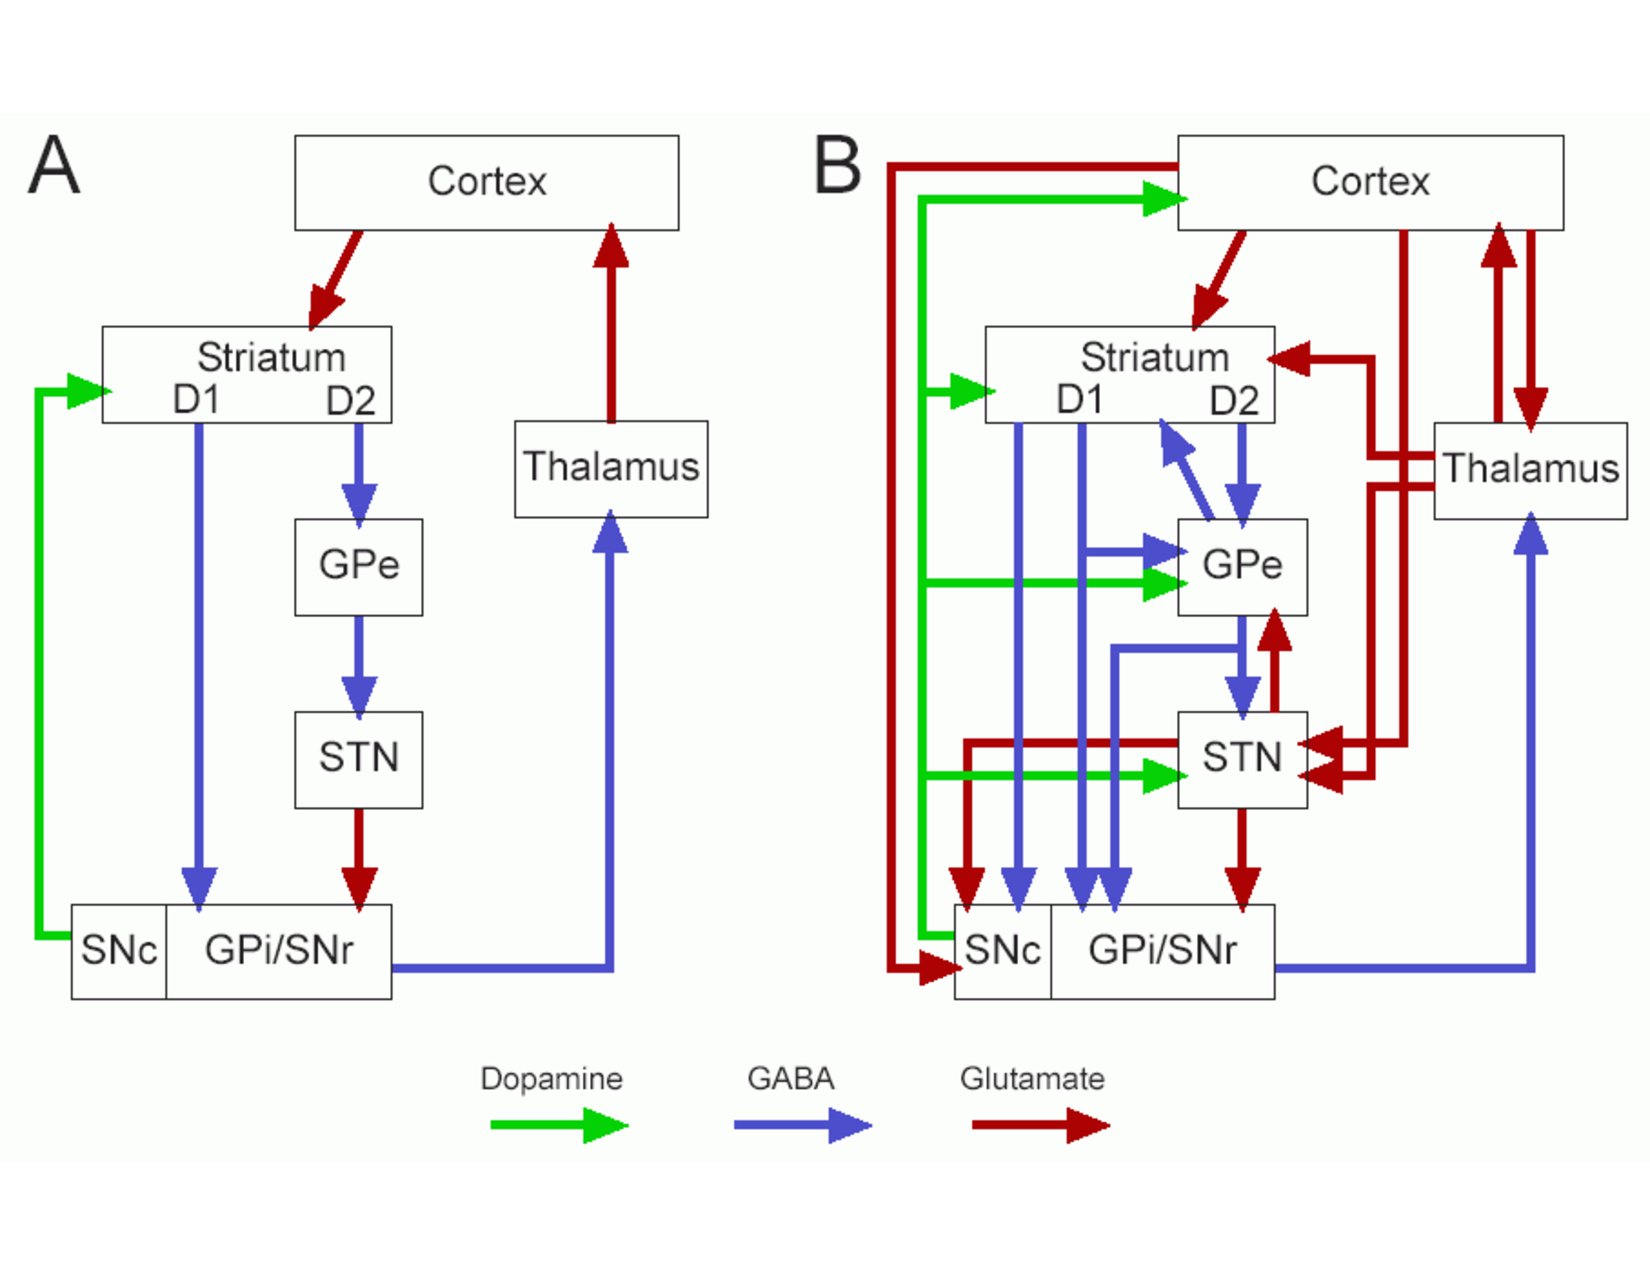
\includegraphics[width=0.8\textwidth]{figures/ch4_4_Bg3}
\end{center}
\caption{Organisation des connexions intrinsèques dans les noyaux gris centraux. A. La proposition influente par Albin et ses collègues (1989). La sortie des ganglions de la base est déterminée par l'équilibre entre les connexions inhibitrices directes (la voie directe) et la voie indirecte via des relais dans le pallidum externe (GPe) et le noyau sous-thalamique (STN). L'équilibre est supposé être réglé par des signaux dopaminergiques afférents de la substance noire compacte (SNc) agissant différemment sur les récepteurs de la dopamine D1 et D2. B. Des études anatomiques récentes ont révélé une organisation un peu plus complexe avec de nouvelles connexions.[Scholarpedia]}
\label{Albin}
\end{figure}

La voie dite ``directe'' est représentée par les projections directes, inhibitrices, GABAergiques du \gls{str} sur la \gls{snr} et le \gls{gpi}. Par cette voie, le striatum inhibe l'activité spontanée, tonique et inhibitrice et également GABAergique des structures de sortie des \gls{bg}. La voie dite ``indirecte'' comporte une étape supplémentaire impliquant successivement le \gls{gpe} et le \gls{stn} puisque le striatum renvoie également des projections GABAergiques inhibitrices vers le \gls{gpe} qui à son tour renvoie des projections GABAergiques inhibitrices vers le \gls{stn}. En inhibant les neurones GABAergiques du GPe, les neurones striataux projettant sur le \gls{gpe} désinhibent donc les neurones glutamatergiques du \gls{stn}. C'est ainsi que les neurones du \gls{stn} renforcent au final l'inhibition tonique que les structures de sortie des \gls{bg} exercent sur leurs cibles grâce à ses projections glutamatergiques excitatrices sur la \gls{snr} et le \gls{gpi}.\\

Il est considéré que la dopamine libérée à partir de la \gls{snc} agit sur deux sous-types de récepteurs dopaminergiques situés au \gls{str} et présentant des effets opposés. La dopamine aurait ainsi un effet global facilitateur sur la voie directe par l'intermédiaire des récepteurs D1 et inhibiteur sur la voie indirecte par l'intermédiaire des récepteurs D2.\\

Ce modèle a été appliqué à des mouvements des membres \cite{Mink:1996} et des mouvements des yeux \cite{Hikosaka:1993}, même si le circuit oculomoteur est un peu différent puisqu'il fait intervenir le colliculus supérieur, structure sous corticale \cite{McHaffie:2005}. Dans sa version de base, ce premier modèle ne prend pas en considération la voie hyper-directe, précédemment évoquée, qui comporte la projection corticale vers le noyau sous-thalamique sans passer par le striatum. Il considère ainsi que ce dernier est l'entrée corticale unique des \gls{bg}. En outre, il a été démontré que ce modèle a plusieurs lacunes et ne répond pas à certaines données cliniques et atomiques \cite{Parent:1998}.\\

En effet ce modèle ``classique'' ne prend en compte qu'une partie des connexions entre les \gls{bg} (fig \ref{Albin}-B) \cite{Parent:1998,Parent:2001}. Il ne considère pas les projections inhibitrices GABAergiques directes du \gls{gpe} sur la \gls{snr} et le \gls{gpi}. De même, il néglige les connexions réciproques entre le \gls{gpe} et le \gls{stn} \cite{Shink:1996}. Il est surtout reproché à ce modèle de considérer que l'information est transmise de manière séquentielle et unidirectionnelle depuis le striatum vers les structures de sortie des \gls{bg}.\\

\subsubsection{Le mod\`ele GPR}

Ensuite \cite{Redgrave:1999} se sont intéressés au rôle des \gls{bg} dans la sélection de l'action chez les vertébrés et ont proposé un modèle qualitatif de l'architecture des noyaux gris centraux. Ils ont expliqué les opérations de sélection de \gls{bg} et décrit le rôle de la dopamine dans le cadre de la sélection de l'action. Ils ont combiné les approches ascendantes (\textit{bottom-up}) et descendantes (\textit{top-down}) dans la modélisation des boucles à travers les noyaux gris centraux. Les modèles de l'approche ascendante partent de données biologiques pour définir l'architecture et les paramètres. En revanche, l'approche descendante part d'un problème comportemental et propose des théories fonctionnelles sur lesquelles seront basés les modèles. Selon leur étude qualitative un système neuronal, tels les \gls{bg}, ne peut être considéré comme le lieu d'un mécanisme de l'\gls{as} que s'il répond aux exigences suivantes: \\

\begin{itemize}
\item le système doit avoir l'information sur les facteurs influant la décision. Ces facteurs peuvent être internes à l'organisme ou provenant de l'environnement extérieur.
\item il faut un paradigme de calcul de la saillance comme ceux cités dans l'introduction.
\item il faut un mécanisme qui permet de résoudre le conflit entre les actions concurrentes. Citons l'exemple de l'inhibition récurrente réciproque. Dans ce mécanisme plusieurs unités connectées s'inhibent mutuellement formant une rétroaction positive. En effet, la hausse d'activité d'une unité provoque l'inhibition des autres et donc la diminution de l'effet inhibiteur de ces derniers sur cette unité et donc la sur-activation de celle-ci. 
\item la sortie du système permet d'exprimer l'action gagnante en éliminant les autres. L'exemple précédent l'assure puisque ce mécanisme permet d'augmenter le contraste entre plusieurs activations concurrentes et assure ainsi le gain de l'activation la plus importante.\\  
\end{itemize}

De nombreux modèles de calcul de \gls{bg} ont été proposés ensuite afin d'étudier le mécanisme de \textit{sélection par désinhibition} \cite{Chevalier:1990} dans les ganglions de la base (pour des revues voir \cite{Gillies:2000, Gurney:2004}). Parmi ceux-ci, nous nous sommes intéressés en particulier au modèle de \cite{Gurney:2001a,Gurney:2001b} qui a été testé comme mécanisme de sélection de l'action pour les agents autonomes en mesure par exemple de résoudre une tâche de survie minimale  \cite{Girard:2003, Girard:2005a, Gonzalez:2000, Prescott:2006}.\\

Les effets de la variation de la dopamine tonique provenant de la [\gls{vta}] sur la sélectivité du modèle ont été examinés \cite{Gurney:2001b} ainsi que son implication dans le contrôle de la balance entre les stratégies d'exploitation et d'exploration dans la sélection de l'action \cite{Humphries:2012}. La dopamine phasique impliquée dans l'apprentissage par renforcement (moduler en temps réel les saillances des actions) n'a pas été considérée et les saillances des actions ont été modulées à la main à partir des entrées sensorielles, proprioceptives et contextuelles.  \\

\begin{figure}
\begin{center}
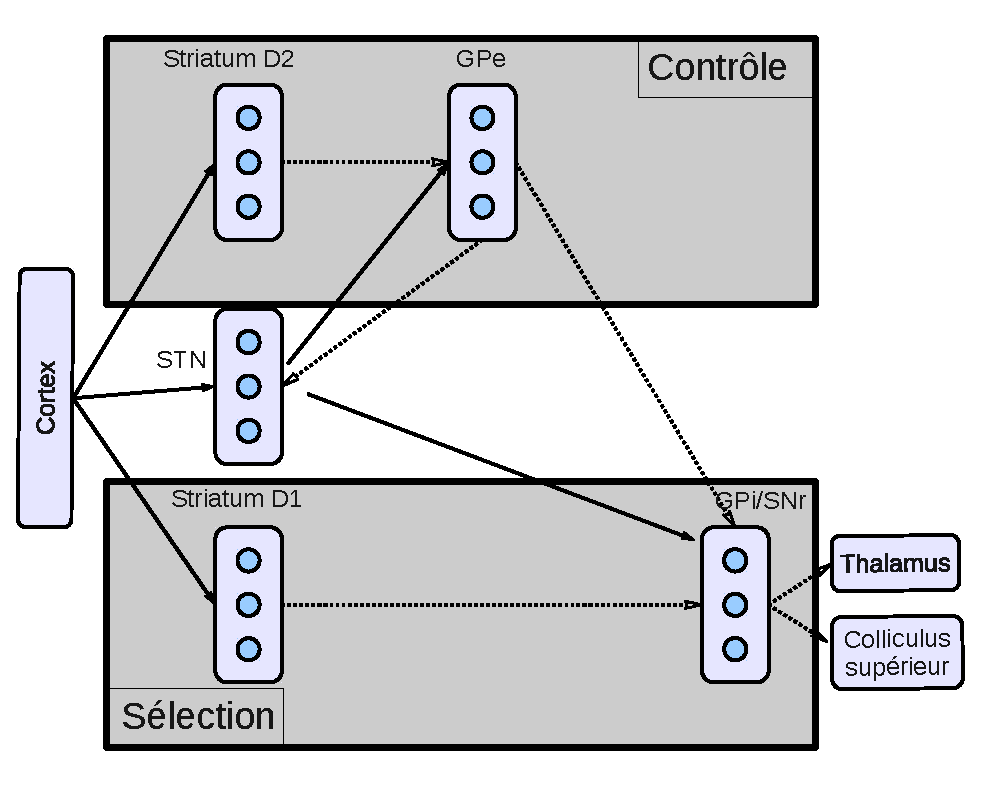
\includegraphics[width=0.7\textwidth]{figures/ch4_5_gpr}
\end{center}
\caption{Les voies de sélection et de contrôle selon le modèle \protect\gls{gpr}. Les flèches pleines: connexions excitatrices. Les flèches en pointillés: connexions inhibitrices. STN: noyau sous-thalamique, Striatum D1: striatum avec récepteurs de dopamine D1, Striatum D2: striatum avec récepteurs de dopamine D2, GPe: pallidum externe, GPi: pallidum interne, SNr: substance noire réticulée. }
\label{GPR}
\end{figure}


Le modèle [\gls{gpr}] a donné une interprétation de l'architecture intrinsèque des \gls{bg} différente de l'interprétation classique basée sur le schéma d'Albin \cite{Albin:1989} (voie directe/voie indirecte). Les auteurs ont ajouté des voies à travers le \gls{gpe}, comme une boucle de régulation qui stabilise les voies de sélection dans les anciens modèles et améliore la sélectivité (fig\ref{GPR}). Ils considèrent donc deux voies, une voie de sélection et une voie de contrôle. La figure (fig. \ref{GPR}) montre les différentes connexions considérées dans le modèle. Les flèches continues représentent les projections excitatrices et les flèches discontinues les projections inhibitrices. Dans un article ultérieur, \cite{Humphries:2002} ont introduit un modèle computationnel du circuit cortico-basal-thalamo-cortical.\\

\subsubsection{Le mod\`ele CBG}

Un modèle modifié de \cite{Gurney:2001a} a été proposé par \cite {Girard:2008} de manière à améliorer ses caractéristiques dynamiques en utilisant la théorie analytique de contraction. En particulier, ce modèle [\gls{cbg}] prend en compte des projections, généralement négligées, entre le \gls{gpe} et le \gls{str} permettant d'améliorer son efficacité. Cette connexion \gls{gpe}-\gls{str} sert à faire taire les neurones striataux non choisis qui est en accord avec le fait que le striatum est connu pour être silencieux au repos \cite{Delong:1984}. Ce modèle néglige les projections du \gls{stn} vers le \gls{str} \cite{Parent:2000} ainsi que les connexions latérales dans le \gls{gpe} et le \gls{snr} \cite{Deniau:1982, Juraska:1977} qui sont ajoutées au modèle \gls{gpr} dans \cite{Gurney:2004}. La figure \ref{CBG} montre les connexions prises en compte par le modèle. Les flèches pleines désignent les connexions inhibitrices et les flèches vides désignent les projections excitatrices.\\

\begin{figure}
\begin{center}
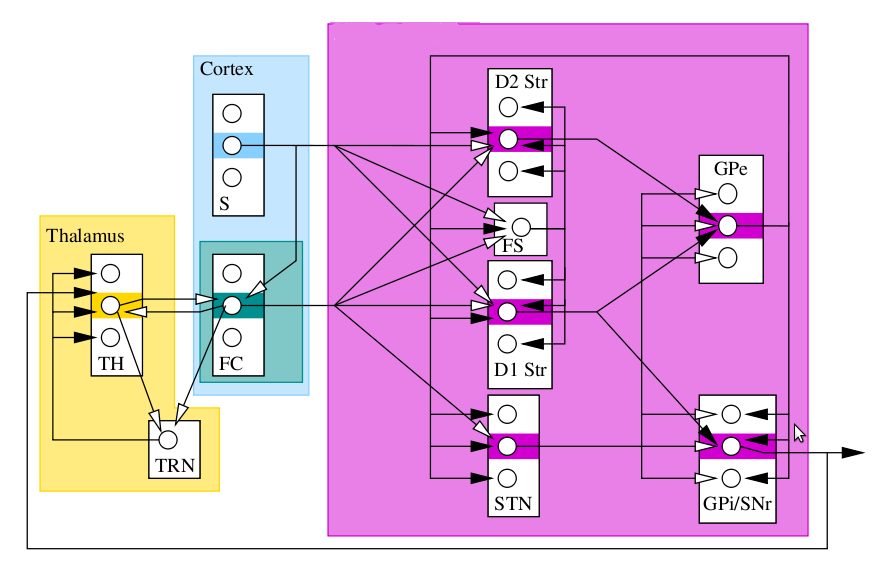
\includegraphics[width=0.8\textwidth]{figures/ch4_6_CBG}
\end{center}
\caption{Le modèle \protect\gls{cbg}. Les flèches pleines désignent les connexions inhibitrices et les flèches vides désignent les projections excitatrices. STN: noyau sous-thalamique, Striatum D1: striatum avec récepteurs de dopamine D1, Striatum D2: striatum avec récepteurs de dopamine D2, GPe: pallidum externe, GPi: pallidum interne, SNr: substance noire réticulée, FS: neurones à décharge rapide (fast spiking) (tiré de \protect\cite{Girard:2008})}
\label{CBG}
\end{figure}

Comme dans le modèle \gls{gpr}, seule la dopamine tonique a été considérée et le mécanisme basique de sélection par désinhibition est conservé. En effet, dans les deux modèles \gls{gpr} et \gls{cbg} la sélection est basée sur des boucles locales récurrentes entre six canaux en compétition. Si l'entrée ne change pas au cours de la simulation, même si on perturbe l'activité au niveau du \gls{str}, le choix est déterministe et donc la saillance de l'action au niveau du \gls{pfc} est déterminante de l'action à choisir ({\em feedforward selection}). 


En s'inspirant de ces deux modèles, nous proposons un nouveau modèle de la boucle motrice des ganglions de la base en leur attribuant un rôle actif dans le calcul de la saillance et par la suite dans la sélection de l'action dépendant du contexte sensoriel, temporel et motivationnel. Nous avons modifié, supprimé et ajouté différentes projections afin de rendre compte du schéma de sélection que nous proposons. Nous détaillerons en premier lieu les caractéristiques de la version basique de notre modèle en le positionnant par rapport aux modèles précédemment évoqués. En deuxième lieu, les résultats des simulations seront discutés en évoquant la version complète utilisant l'apprentissage.\\  

\section{Conception et modélisation}

Le modèle de sélection motivée de l'action que nous proposons, inspiré des modèles \cite{Gurney:2001a, Girard:2008}, conserve le mécanisme basique de sélection intrinsèque par désinhibition. L'interaction entre plusieurs flux et différentes boucles récurrentes permettant de mettre en compétition une excitation diffuse et une inhibition locale à travers les différentes voies rend complexe la mise en oeuvre d'un modèle adaptatif et encore plus difficile la description de sa dynamique.\\
 
Nous proposons en particulier deux mécanismes supplémentaires. D'abord, un mécanisme d'évaluation de la saillance donne plus de liberté dans la détermination du choix de l'action, en considérant en particulier un feedback thalamique souvent négligé dans les boucles cortico-basales vers le striatum. Ce mécanisme permet de mettre en compétition ce qui est appris par l'habitude (projection cortex-cortex), ce qui est choisi par exploration (projection cortex-striatum) et ce qui est choisi par motivation (projection contexte-striatum). Ensuite, nous avons a mis en oeuvre un mécanisme adaptatif de création dynamique d'une représentaion du contexte (structure S), donc de création de méta-actions en faveur de l'approche énactive.\\%résultats

\subsection{Hypothèses}

L'architecture de base de notre modèle est similaire à celle de \cite{Gurney:2001a, Gurney:2001b, Girard:2005a, Girard:2008}. Nous utilisons le même type de neurones (intégrateur à fuite voir section 1) et chaque canal de \gls{bg} est représenté par une unité dans chacun des noyaux. On se situe donc dans le circuit moteur, chaque canal correspond donc à une action motrice.\\ 

Une différence principale par rapport à ces modèles est l'entrée du système qui n'est plus un vecteur pré-calculé de saillances. C'est un vecteur de perception sensorielle auquel est associé une pré-activation motrice correspondant aux actions candidates, réalisée par une sorte de mémoire de travail\footnote{C'est la capacit\'e \`a maintenir et \`a utiliser des repr\'esentations mentales pour les comportements orient\'es vers un but. Le cortex pr\'efrontal est réputé pouvoir réaliser des fonctions de m\'emoire de travail \cite{Petrides:1994, Cohen:1997}. Les \gls{bg} aussi, support\'es par des connexions anatomiques avec les aires corticales associatives.}. %Middelton_1994,Levy_1997,Owen_1996,Owen_1999}.
Une entrée représentant un contexte supplémentaire sera ajoutée dans une version traitée plus tard qui servira à apprendre à choisir des actions en fonction d'une consigne particulière et non pas seulement en fonction de son importance dans la mémoire de travail.\\

En effet, le cortex pariétal postérieur [\gls{ppc}] participe à l'évaluation du contexte sensoriel dans lequel s'effectue le mouvement. Le cortex pariétal évalue les différentes données comme la position du corps et de la cible dans l'espace grâce aux informations somatosensorielles, proprioceptives et visuelles qu’il reçoit. Il produit ainsi des modèles internes du mouvement à effectuer vers le cortex prefrontal [\gls{pfc}], en amont des cortex prémoteur et moteur. Ainsi dans notre modèle, une tâche de sélection commence par l'activation d'une unité du \gls{ppc} correspondant à un perception sensorielle donnée, qui à son tour, active un sous ensemble des unités du \gls{pfc} de manière inégale. Chaque unité active dans le \gls{pfc} correspond à une action candidate et une activation plus importante qu'une autre signifie que l'action concernée a été plus utilisée dans l'histoire et l'expérience de l'agent (les poids de projections entre le \gls{ppc} et le \gls{pfc} sont supposés être appris grâce à une règle hebbienne\footnote{Loi de Hebb :la force de la connexion (synaptique) présente entre deux neurones est augmentée durablement lorsque la décharge du neurone pré-synaptique (en amont de la synapse) est fortement corrélée temporellement à celle du neurone post-synaptique (en aval de la synapse) \cite{Hebb:1949}}).\\

L'hypothèse de fonctionnement en bandes parallèles dans les \gls{bg} se base sur un effet macroscopique. Comme il est nécessaire que les différents circuits impliquant les \gls{bg} communiquent, on peut supposer qu'au sein d'un circuit les canaux peuvent se rejoindre comme au niveau du \gls{stn} et on peut utiliser des projections diffuses du \gls{ppc} vers le \gls{str} (i.e. le \gls{ppc} renvoie une excitation supplémentaire vers toutes les cellules striatales). Nous supposons que cette projection corticale prépare l'activation d'unités striatales qui correspondent aux actions candidates. En effet, le \gls{str} est toniquement silencieux et a donc besoin d'être fortement stimulé pour que les neurones striataux arrivent à leur seuil d'activation. Il reçoit aussi des projections excitatrices du \gls{pfc}. \\ 

On ne distingue pas les neurones selon leurs sensibilités à la dopamine donc on ne considérera pas de subdivisions internes au striatum. En effet, on ne s'intéresse pas à la dopamine tonique ce qui revient à moduler les poids des projections entre le \gls{str} d'une part et le \gls{gpe} et le \gls{gpi} d'une autre part. En plus les neurones qui projettent vers le \gls{gpi} et le \gls{gpe} sont morphologiquement et topographiquement indifférenciables dans le \gls{str} donc on a choisi de ne pas tenir compte de la différence des récepteurs de dopamine \cite{Gerfen:1990} (d'autant plus que ce sujet est controversé dans la littérature). Le \gls{str} reçoit aussi des projections excitatrices du \gls{pfc}, d'autres inhibitrices du \gls{gpe}. On suppose en plus la présence d'une activité parasite faible, un bruit $N$  qui vient perturber l'activité striatale sans pouvoir dépasser le seuil d'activation $e_{\gls{str}} $. Ainsi l'entrée du \gls{str} est décrite par l'équation suivante. Nous avons ajouté un feedback thalamique provenant plus particulièrement du thalamus ventro-latéral [\gls{vlt}] ${\gls{vlt}}_{Out}$  qui va renforcer le choix fait par la partie intrinsèque des ganglions de la base, qui peut être différent de celui pré-imposé par la pré-activation au niveau du \gls{pfc}.\\

\begin{center}
\begin{equation} 
\gls{str}_{In}= {\gls{ppc}}_{Out}+{\gls{pfc}}_{Out}-{\gls{gpe}}_{Out}+{\gls{vlt}}_{Out}-e_{\gls{str}}+N
\end{equation}
\label{eqstr}
\end{center}

En effet, dans les modèles \gls{gpr} et \gls{cbg} la sélection est déterministe, le plus fort gagne la compétition. Pour passer à une sélection active et pouvoir intégrer un mécanisme d'apprentissage, un retour post-moteur est nécessaire d'où l'intérêt d'intégrer la projection excitatrice glutamatergique des noyaux thalamiques vers le \gls{str} \cite{Lapper:1992, Sadikot:1992}.\\

D'autre part, nous avons ajouté une inhibition latérale $L$ lente au niveau du \gls{pfc} qui va s'ajouter à l'excitation récurrente avec le thalamus pour finalement permettre d'avoir à la fin de la simulation une seule action active (prémotrice). Ceci permet d'installer un apprentissage hebbien entre le \gls{ppc} et le \gls{pfc} d'une part et d'autre part renforce la sélection au niveau du \gls{str} et permet d'installer un apprentissage par renforcement en se basant sur la sortie du \gls{str} et non pas seulement sur la sortie du \gls{gpi}. Globalement, à la différence de \gls{gpr} et \gls{cbg}, nous visons une sélection nette à tous les niveaux de la boucle et non pas seulement au niveau du \gls{gpi}. D'où l'équation de l'entrée du \gls{pfc}:

\begin{center}
\begin{equation} 
{\gls{pfc}}_{In}= {\gls{ppc}}_{Out}+{\gls{vlt}}_{Out}-e_{\gls{pfc}}+L
 \end{equation}
\end{center}

Comme dans le modèle \gls{cbg}, le noyau sous-thalamique reçoit seulement du \gls{pfc}, entrée excitatrice des aires motrices du lobe frontal \cite{Mink:1996} et le \gls{str} reçoit de toutes les aires du cortex cérébral \cite{Cherubini:1988, Kemp:1970}. Il reçoit aussi des projections inhibitrices du \gls{gpe}. Son activité tonique est modulée par un seuil d'activation négatif $e_{\gls{stn}}$ d'ou l'équation suivante:

\begin{center}
\begin{equation} 
{\gls{stn}}_{In}= {\gls{pfc}}_{Out}-{\gls{gpe}}_{Out}-e_{\gls{stn}}
 \end{equation}
\end{center}

Le \gls{gpe} et le \gls{gpi} sont des noyaux inhibiteurs. De même que dans \gls{cbg} et \gls{gpr}, ils reçoivent des afférences sélectives du \gls{str} et une
excitation diffuse du \gls{stn}. On néglige la projection entre le \gls{gpe} et le \gls{gpi} puisque la sortie GABAergique inhibitrice du \gls{gpe} est majoritairement vers le \gls{stn} \cite{Rouzaire:1980} et le fait de l'ajouter ne modifie pas les résultats des simulations puisque les poids peuvent être réadaptés: 

\begin{center}
\begin{equation} 
{\gls{gpe}}_{In}= {\gls{stn}}_{Out}-{\gls{str}}_{Out}-e_{\gls{gpe}}
 \end{equation}
\begin{equation} 
{\gls{gpi}}_{In}= {\gls{stn}}_{Out}-{\gls{str}}_{Out}-e_{\gls{gpi}}
 \end{equation}
\end{center}

Le \gls{gpi} et la \gls{snr} sont considérés comme une seule structure fonctionnelle de sortie puisqu'elles possèdent des neurones similaires et historiquement étaient une seule entité \cite{Carpenter:1981}. Et finalement l'équation du noyau \gls{vlt} qui est sous inhibition tonique du \gls{gpi} et en excitation réciproque avec le \gls{pfc} s'écrit:

\begin{center}
\begin{equation} 
{\gls{vlt}}_{In}= {\gls{pfc}}_{Out}-{\gls{gpi}}_{Out}-e_{\gls{vlt}}
 \end{equation}
\end{center}

Il en résulte donc l'architecture présentée dans la figure \ref{TBG0}.

\begin{figure}
\begin{center}
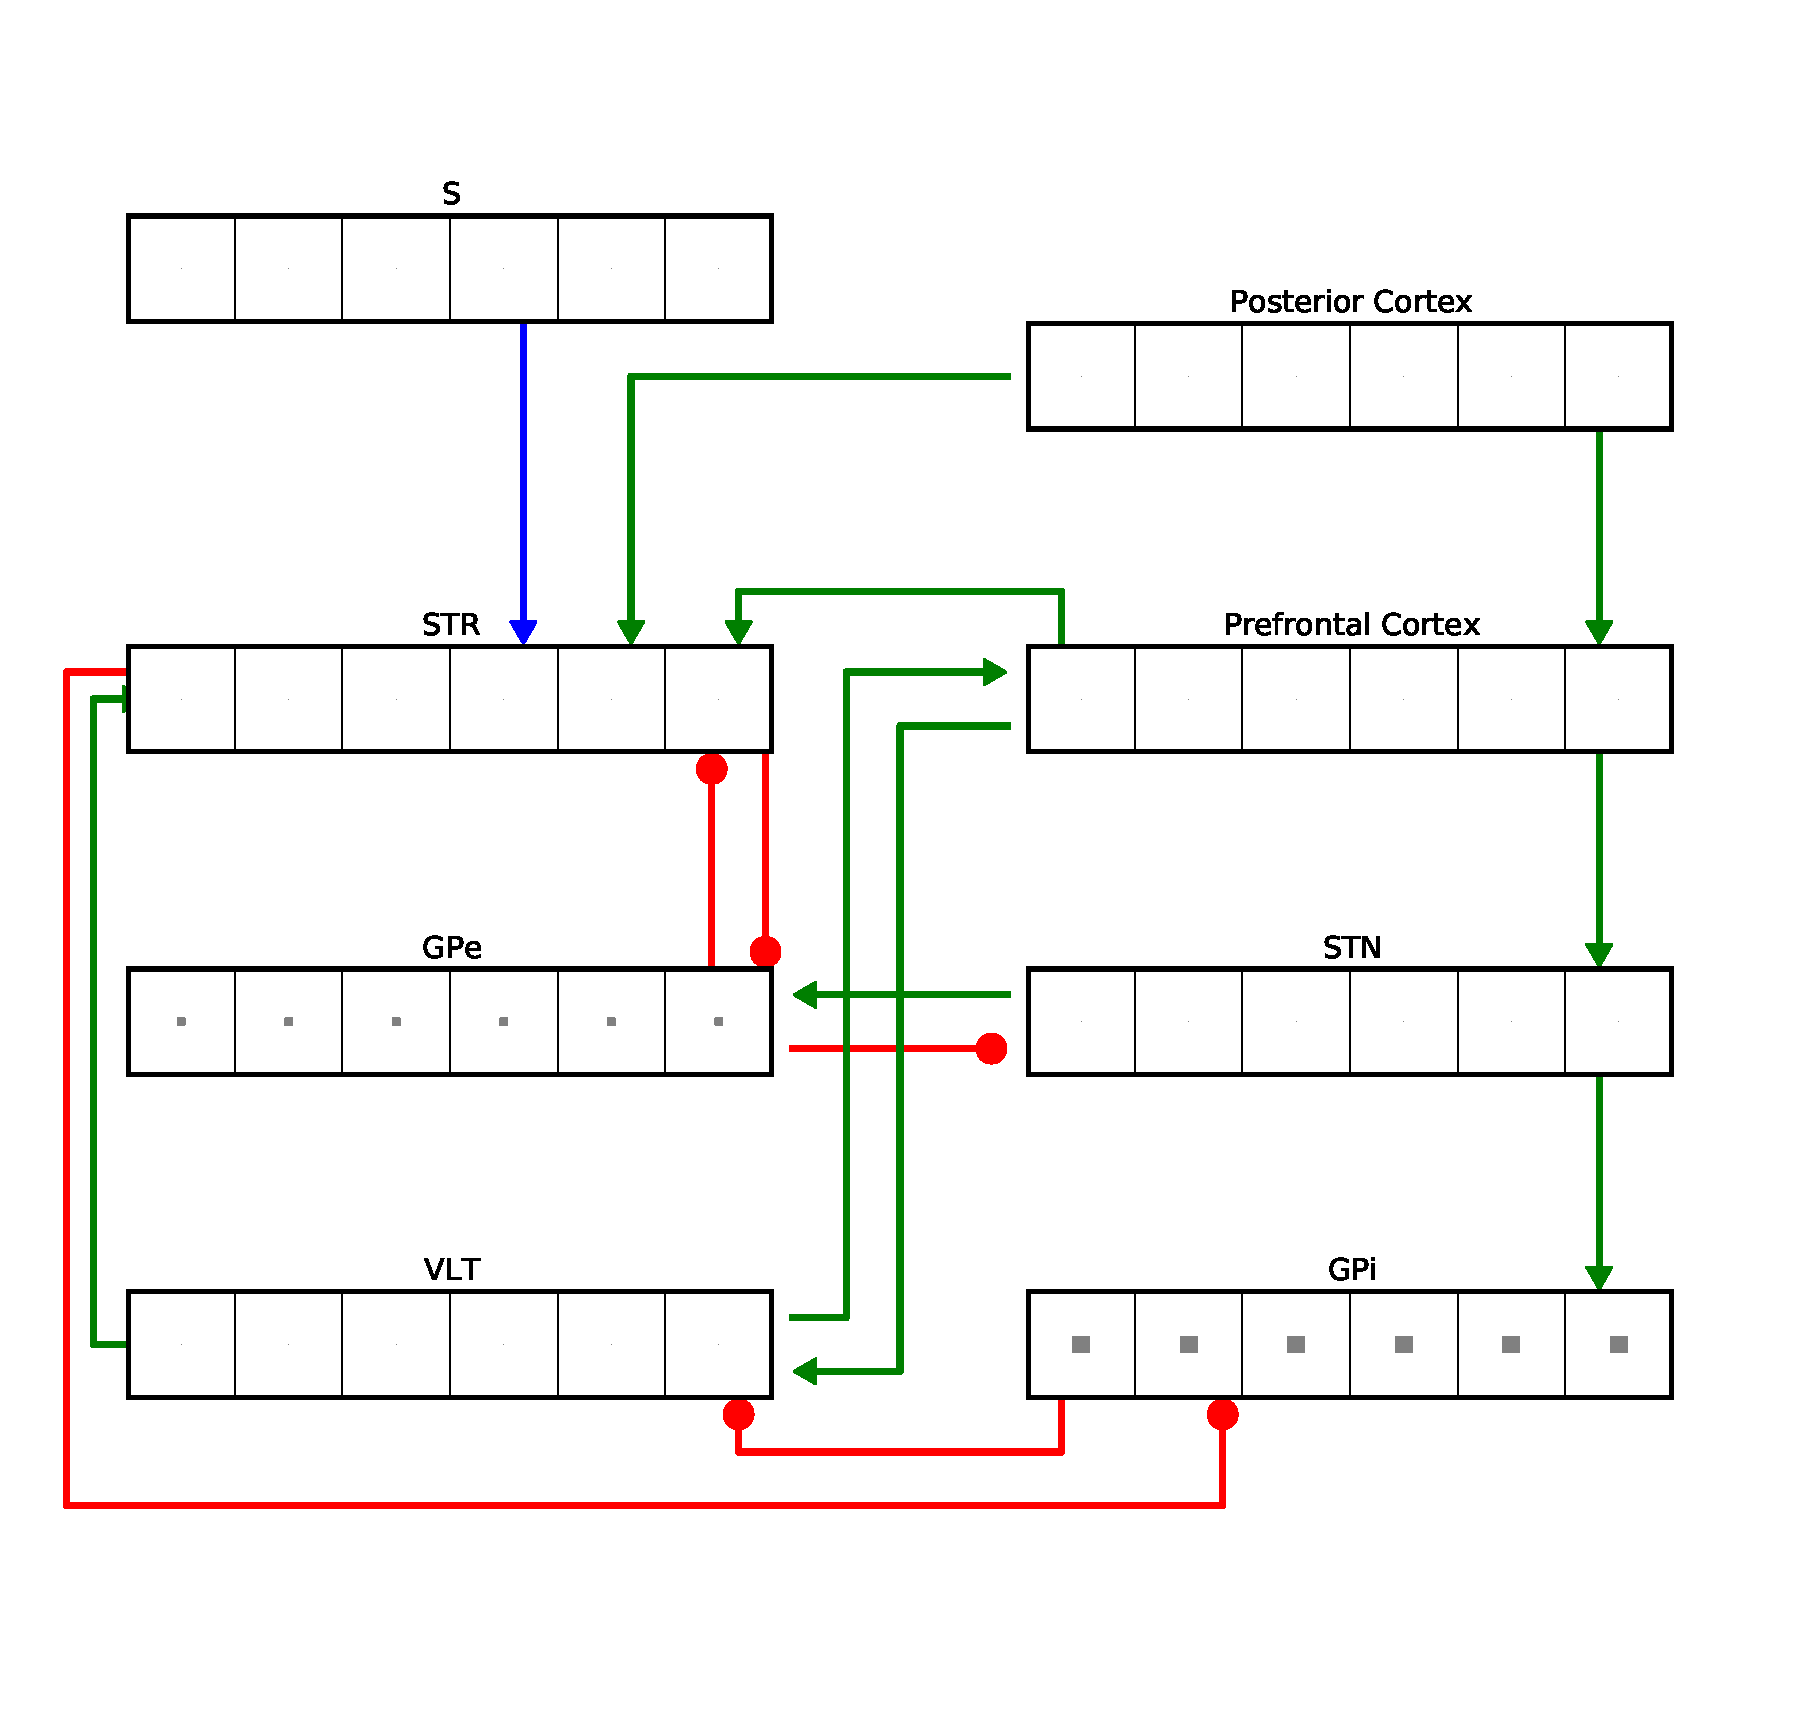
\includegraphics[width=0.5\textwidth]{figures/ch4_7_TBG_00}
\end{center}
\caption{L'architecture de notre modèle de la boucle cortico-basale. Les connexions excitatrices (glutamergiques) sont représentées par des flèches pleines, les connexions inhibitrices (GABAergiques) par des flèches en pointes rondes. En l'absence de stimuli, donc au repos, le \protect\gls{gpe} et le \protect\gls{gpi} sont toniquement actifs. La struture S sera décrite dans la suite.}
\label{TBG0}
\end{figure} 

\subsection{Simulation et résultats}

\subsubsection{Scénario sans apprentissage}

De même que pour les simulations effectuées par les auteurs de modèles \gls{gpr} et \gls{cbg}, nous avons utilisé un modèle à six canaux. Les paramètres ont été fixés à des valeurs résumées en annexe. La simulation a été programmée en python, en utilisant la simple approximation d'Euler (voir chapitre 1) pour l'intégration, avec un pas de temps de 1 ms. \\

Nous avons simulé avec notre modèle un test de sélection simple similaire à celui de \cite{Gurney:2001b} et avec la version du modèle \gls{gpr} présentée dans \cite{Prescott:2006} et reproduite dans \cite{Girard:2008}. La sélection concerne deux canaux d'actions dont les pré-activations au niveau du \gls{pfc} valent 0.4 et 0.6 via une activation du \gls{ppc}. Une simulation dure 2 secondes suivie de 2 secondes de repos pour éviter l'effet de mémoire courte (l'activité forte d'un canal est maintenue jusqu'à ce que le stimulus soit enlevé, et donc peut influencer la prochaine sélection). On représente la même entrée plusieurs fois et on enregistre les profils d'activités des canaux concernés (fig \ref{TBG4}). Nous avons fait un test semblable en implémentant les deux modèles \gls{gpr} (fig \ref{GPR4})et \gls{cbg} (fig \ref{CBG4}) avec la même séquence de simulation et un vecteur de saillance d'entrée (0.4,0.6,0,0,0,0) pour comparer les effets.\\
\begin{figure}
\begin{center}
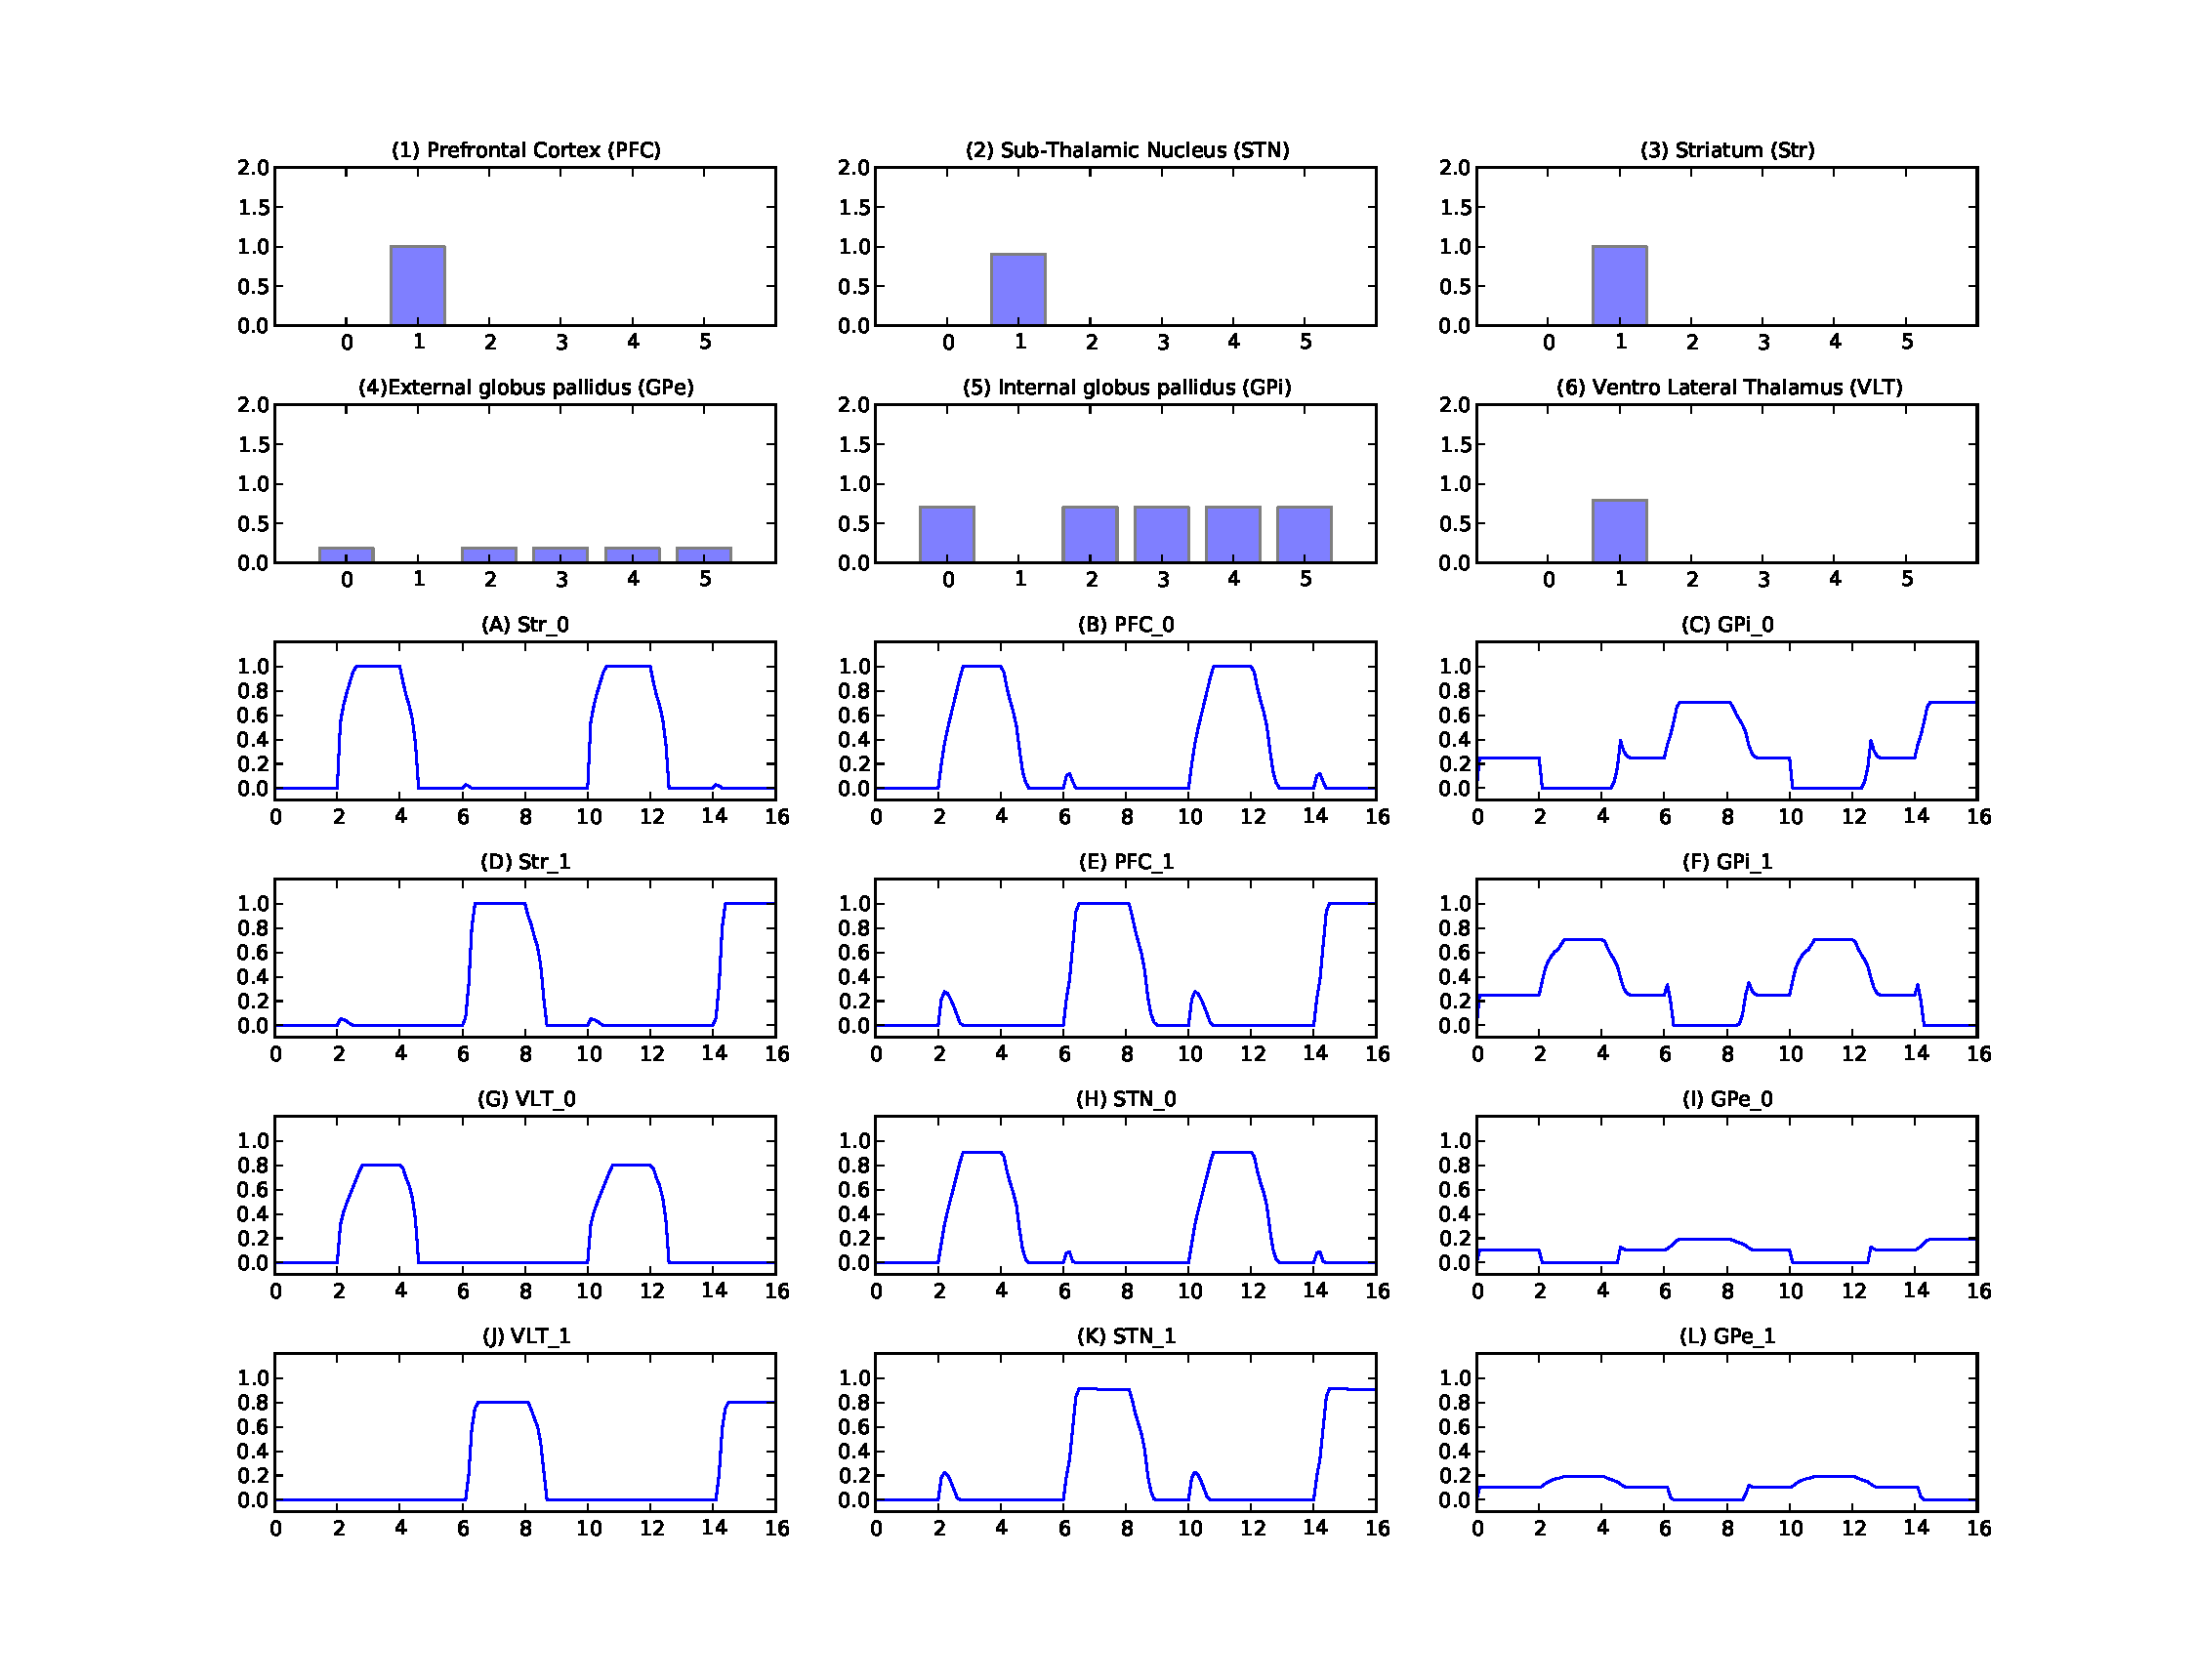
\includegraphics[width=\textwidth]{figures/ch4_8_model_04}
\caption{ Test de sélection entre deux canaux par notre modèle. L'entrée du modèle: On suppose qu'une cellule (la première par exemple) de PC est activée à 1 (n'est pas représentée dans les figures) et qui projette sur PFC avec deux poids différents sur les canaux 0 et 1 (0.4 pour le canal 0 et 0.6 pour le canal 1). Les courbes (A,B,C,D,E,F,G,H,I,J,K,L) représentent l'évolution de l'activité dans le temps dans les deux premiers canaux (lieux de compétition) qui commence par une période de repos (entrée nulle pendant 2s) suivie de 4 simulations (de durée 2s) alternées avec des périodes de repos. Les diagrammes (1,2,3,4,5,6) représentent les niveaux d'activités à la fin d'une simulation dans les 6 unités de chaque structure (les niveaux d'activités sont entre 0 et 1). }
\label{TBG4}
\end{center}
\end{figure}
\begin{figure}
\begin{center}
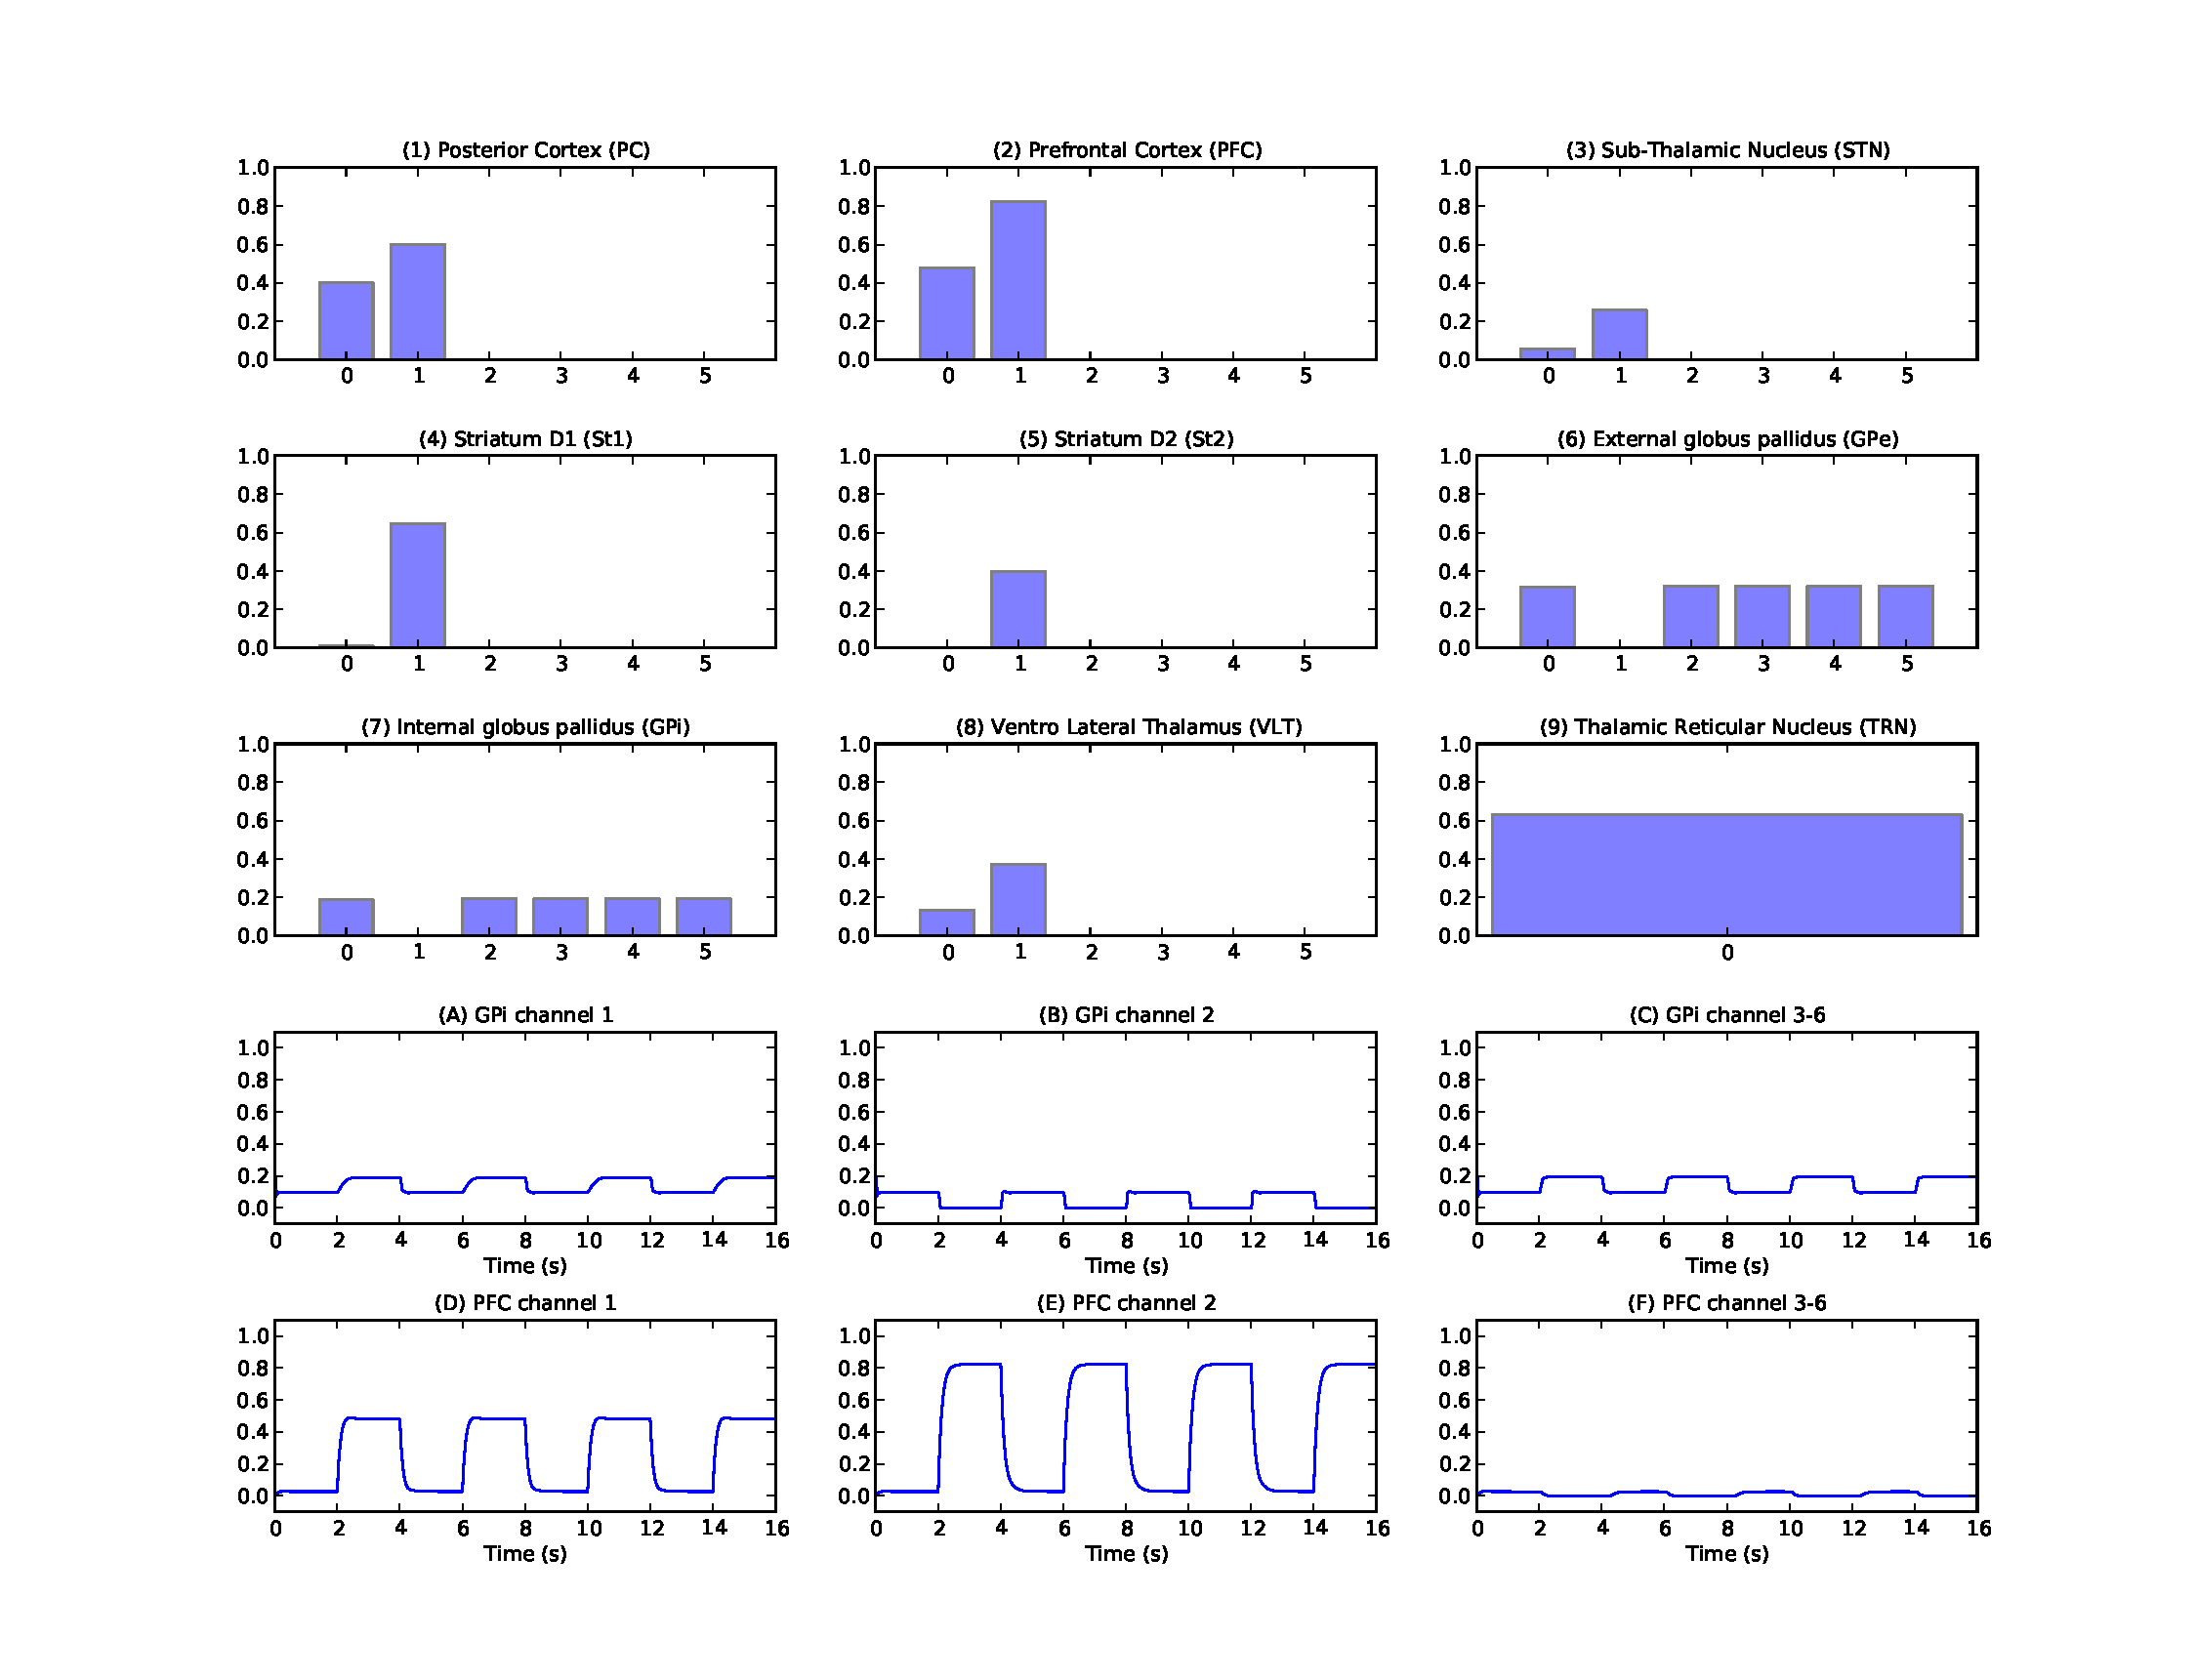
\includegraphics[width=\textwidth]{figures/ch4_9_girard_04}
\caption{ Test de sélection entre deux canaux par le modèle \protect\gls{cbg}. L'entrée du modèle: les deux premiers canaux de PC sont activés à 0.4 et 0.6 simultanément. Les courbes (A,B,C,D,E,F) représentent l'évolution de l'activité dans le temps dans les trois premiers canaux au niveau de \protect\gls{gpi} et \protect\gls{pfc} qui commence par une période de repos (entrée nulle pendant 2s) suivie de 4 simulations (de durée 2s) alternées avec des périodes de repos. Les diagrammes (1,2,3,4,5,6,7,8,9) représentent les niveaux d'activités à la fin d'une simulation dans les 6 unités de chaque structure.}
\label{CBG4}
\end{center}
\end{figure}
\begin{figure}
\begin{center}
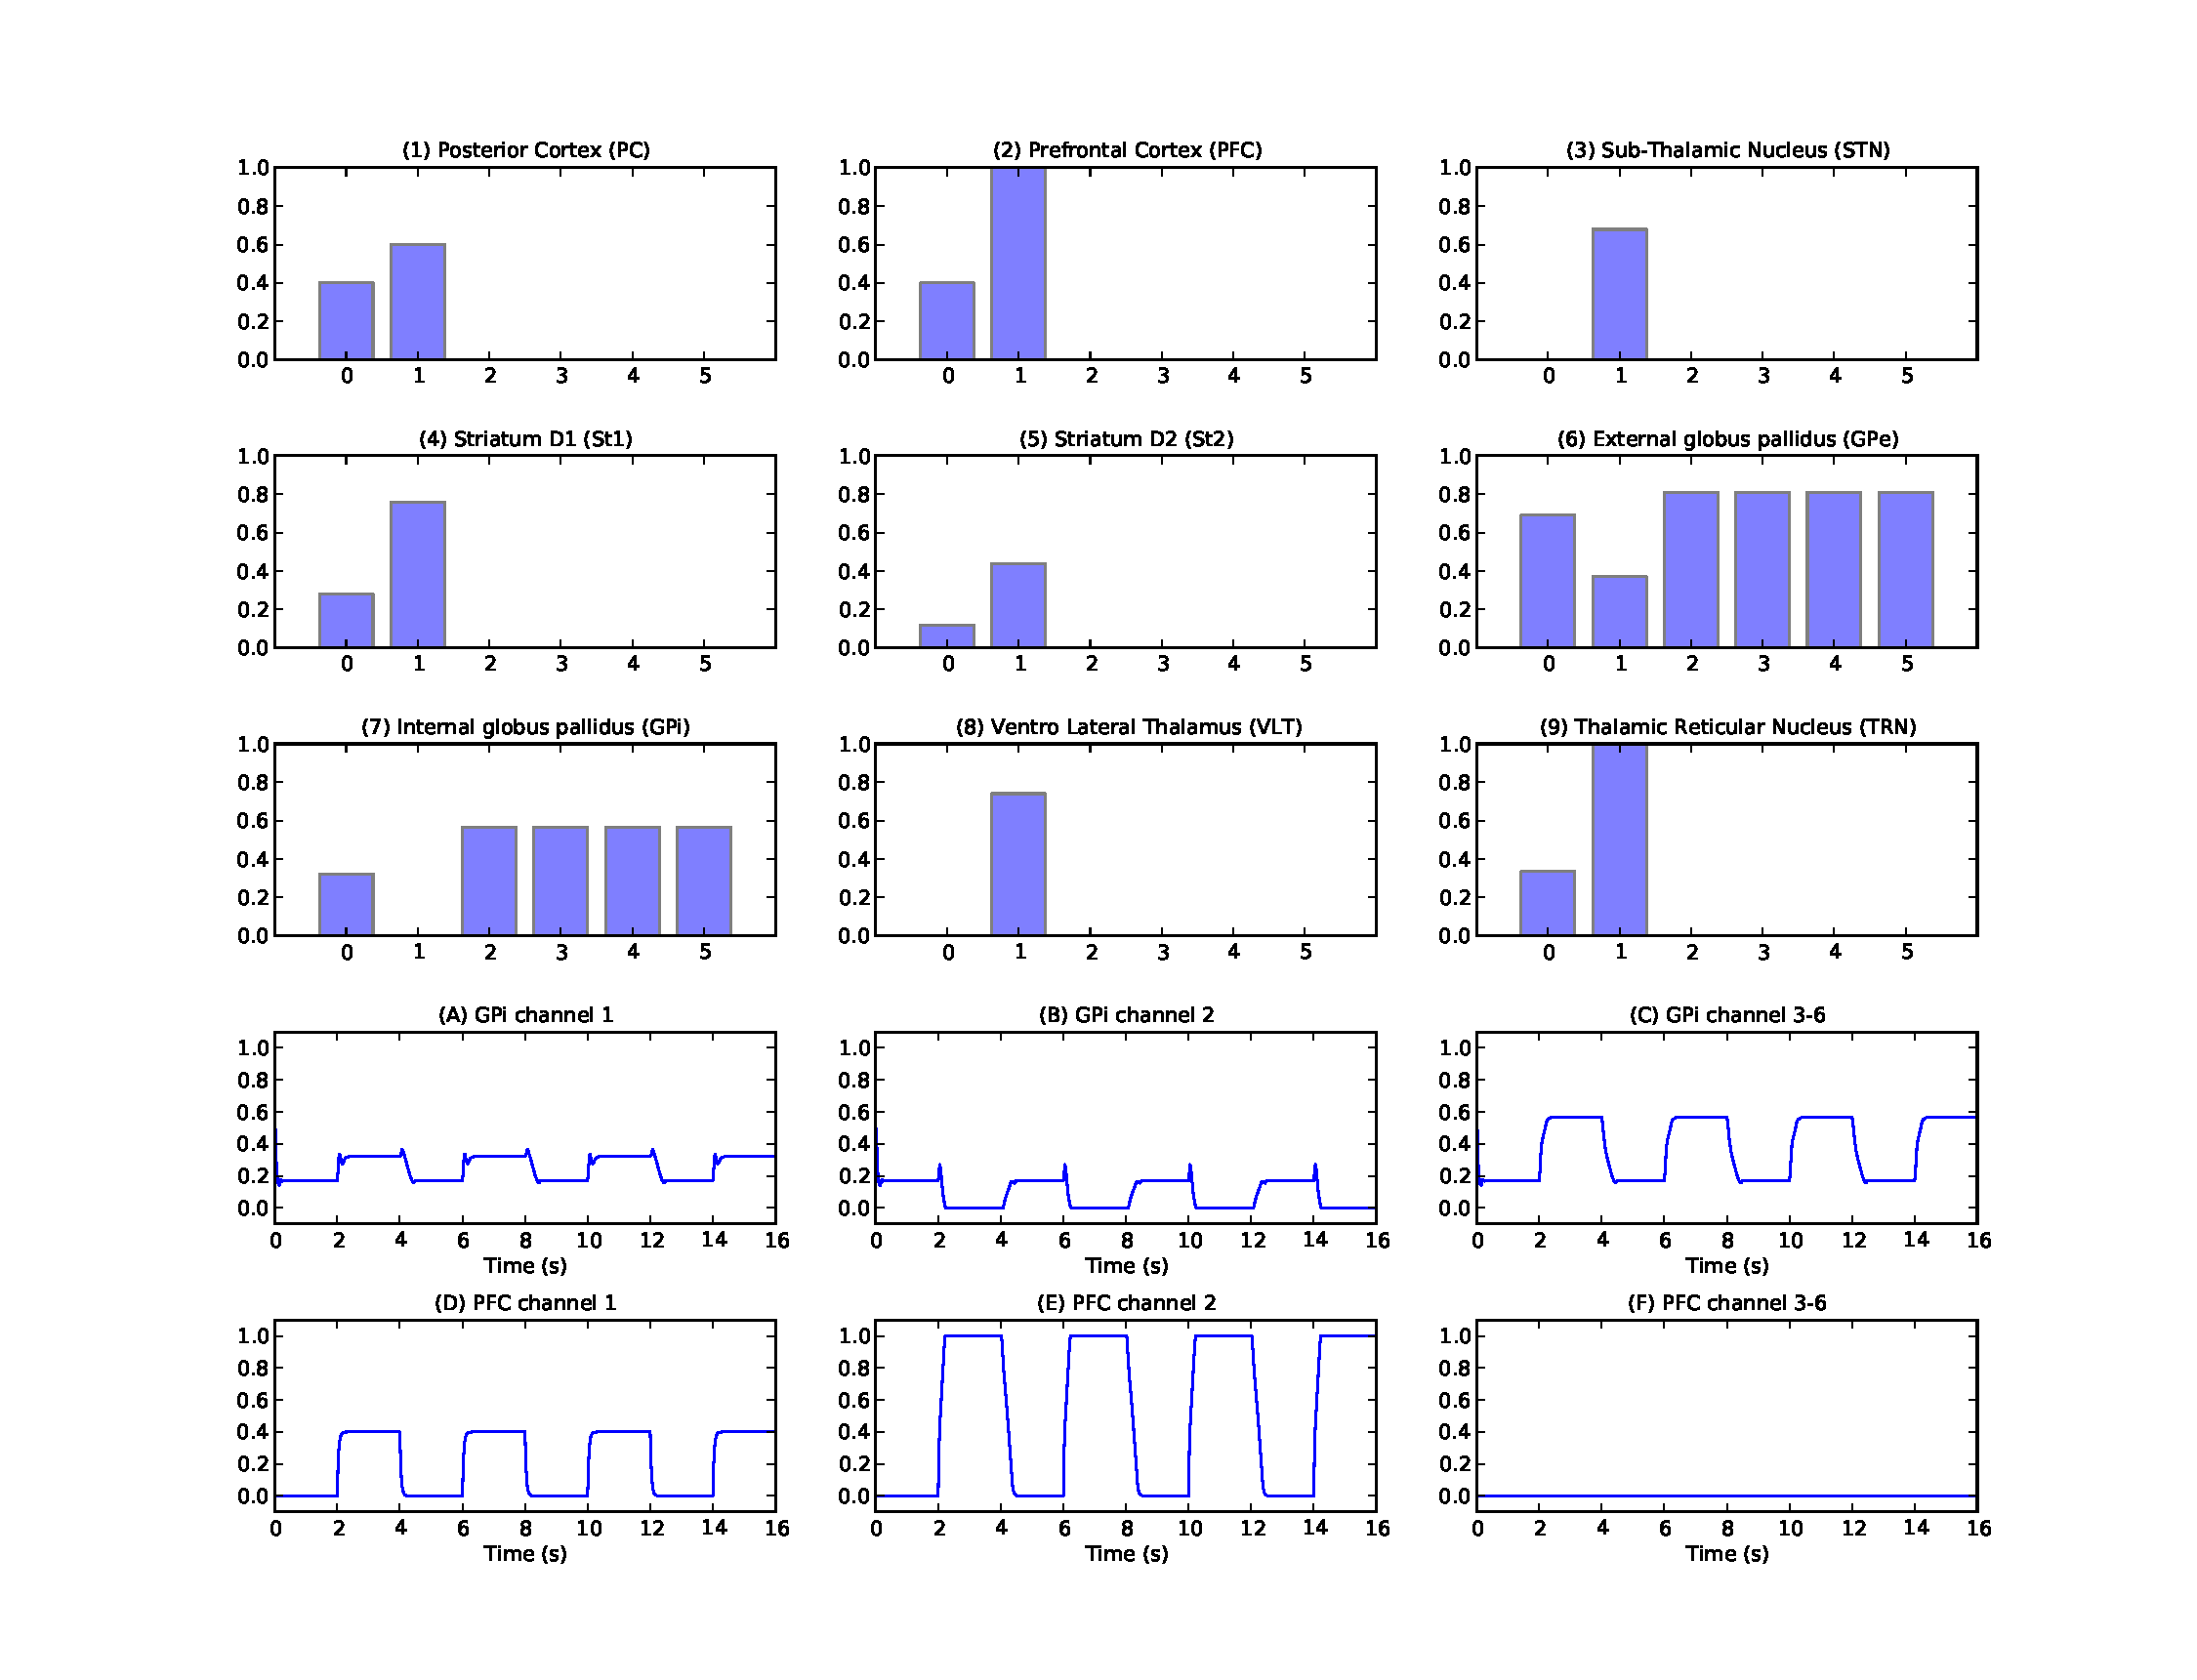
\includegraphics[width=\textwidth]{figures/ch4_10_gurney_04}
\caption{ Test de sélection entre deux canaux par le modèle \protect\gls{gpr}. L'entrée du modèle: les deux premiers canaux de PC sont activés à 0.4 et 0.6 simultanément. Les courbes (A,B,C,D,E,F) représentent l'évolution de l'activité dans le temps dans les trois premiers canaux au niveau de \protect\gls{gpi} et \protect\gls{pfc} qui commence par une période de repos (entrée nulle pendant 2s) suivie de 4 simulations (de durée 2s) alternées avec des périodes de repos. Les diagrammes (1,2,3,4,5,6,7,8,9) représentent les niveaux d'activités à la fin d'une simulation dans les 6 unités de chaque structure.}
\label{GPR4}
\end{center}
\end{figure}

En comparant les diagrammes d'activités à la fin de chaque période de simulation dans les trois modèles, on remarque qu'à la différence des deux autres modèles, dans notre modèle la sélection est nette dans toutes les structures surtout au niveau du \gls{str} et du cortex préfrontal résultant des feedbacks provenant du thalamus et accentuée par l'inhibition latérale au niveau du \gls{pfc}. L'utilité d'avoir une image de sortie de la sélection (\gls{gpi}) est de pouvoir expliciter un apprentissage de poids projetant vers le \gls{pfc} et vers le \gls{str} (voir la sous-section suivante).\\

Dans les modèles \gls{gpr} et \gls{cbg}, l'information la plus étudiée est la sortie du \gls{gpi}. Nous proposons de comparer les profils d'activité du \gls{gpi} dans les deux premiers canaux (les courbes \gls{gpi}-0 et \gls{gpi}-1 dans la figure \ref{TBG4} et les courbes \gls{gpi} channel 1 et \gls{gpi} channel 2 dans les figures \ref{CBG4} et \ref{GPR4}. Prenons par exemple la première simulation entre les dates 2s et 4s. Dans le modèle \gls{cbg} une seule phase (de décroissance) existe avant le retour à l'état d'équilibre, dans le modèle \gls{gpr} on remarque l'existence de deux phases, une augmentation brève de l'activité dans les deux canaux résultant de l'excitation diffuse du \gls{stn} suivie d'une décroissance dans le canal sélectionné. Par contre dans notre modèle, on peut constater sur certaines périodes (courbe \gls{gpi}-1 entre 6 et 8s) trois phases, les deux premières similaires au fonctionnement GPR et une dernière phase de sur-activation du \gls{gpi} avant le retour au niveau tonique. Cette observation est en accord avec les enregistrements neurologiques effectués dans le \gls{gpi} \cite{Nambu:2000} et permet d'apporter un éclaircissement sur la coordination entre les différentes voies dans les ganglions de la base.\\

Une autre différence visible sur les courbes est relative au fait que le choix n'est plus déterministe dans notre modèle. Ce degré de liberté est apporté à ce stade simplement par un bruit ajouté au niveau du \gls{str} pendant une seconde puis enlevé dans chaque simulation. Un tel bruit ne permet pas de modifier la sortie des \gls{bg} dans les deux autres modèles puisque d'une part la saillance est calculée en amont, et d'autre part il y a absence de feedback. Nous nous sommes intéressés en particulier au cas o\`u le premier canal est choisi bien que sa pré-activation initiale (\gls{pfc}) soit moins importante que celle du deuxième canal. La figure \ref{Select} donne une vision globale de l'évolution de l'activité dans les différentes structures avant d'arriver au résultat final.

\begin{figure}

\begin{tabular}{|c|c|}
\hline
t=0.70s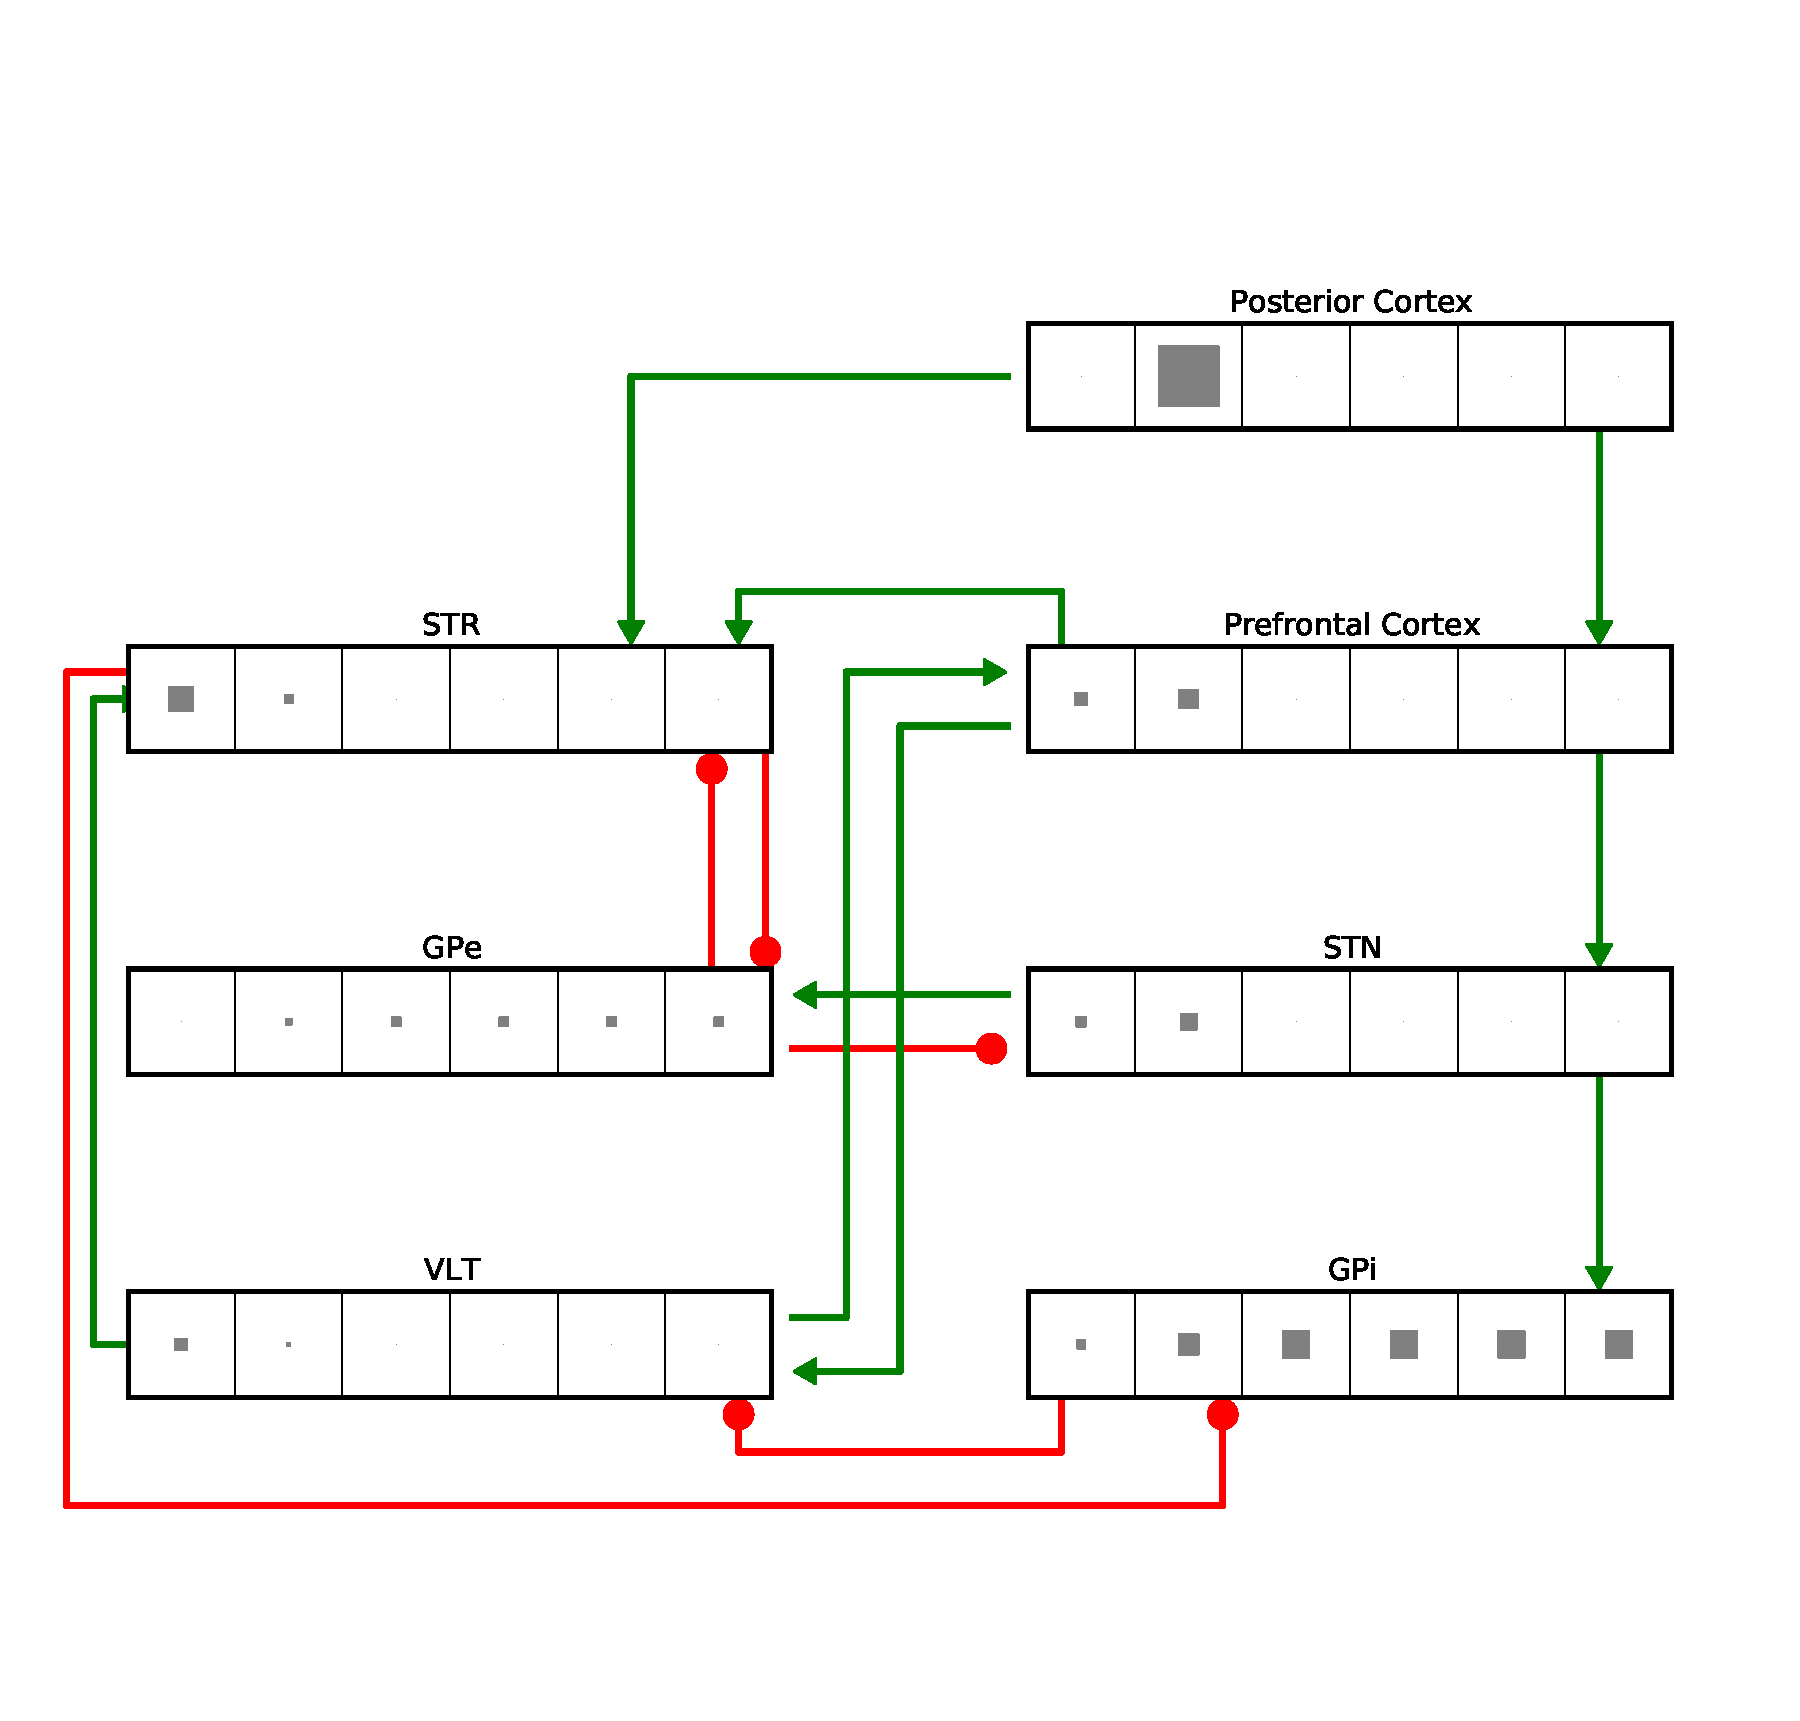
\includegraphics[width=0.4\textwidth]{figures/ch4_11_TBG07}&
t=1.00s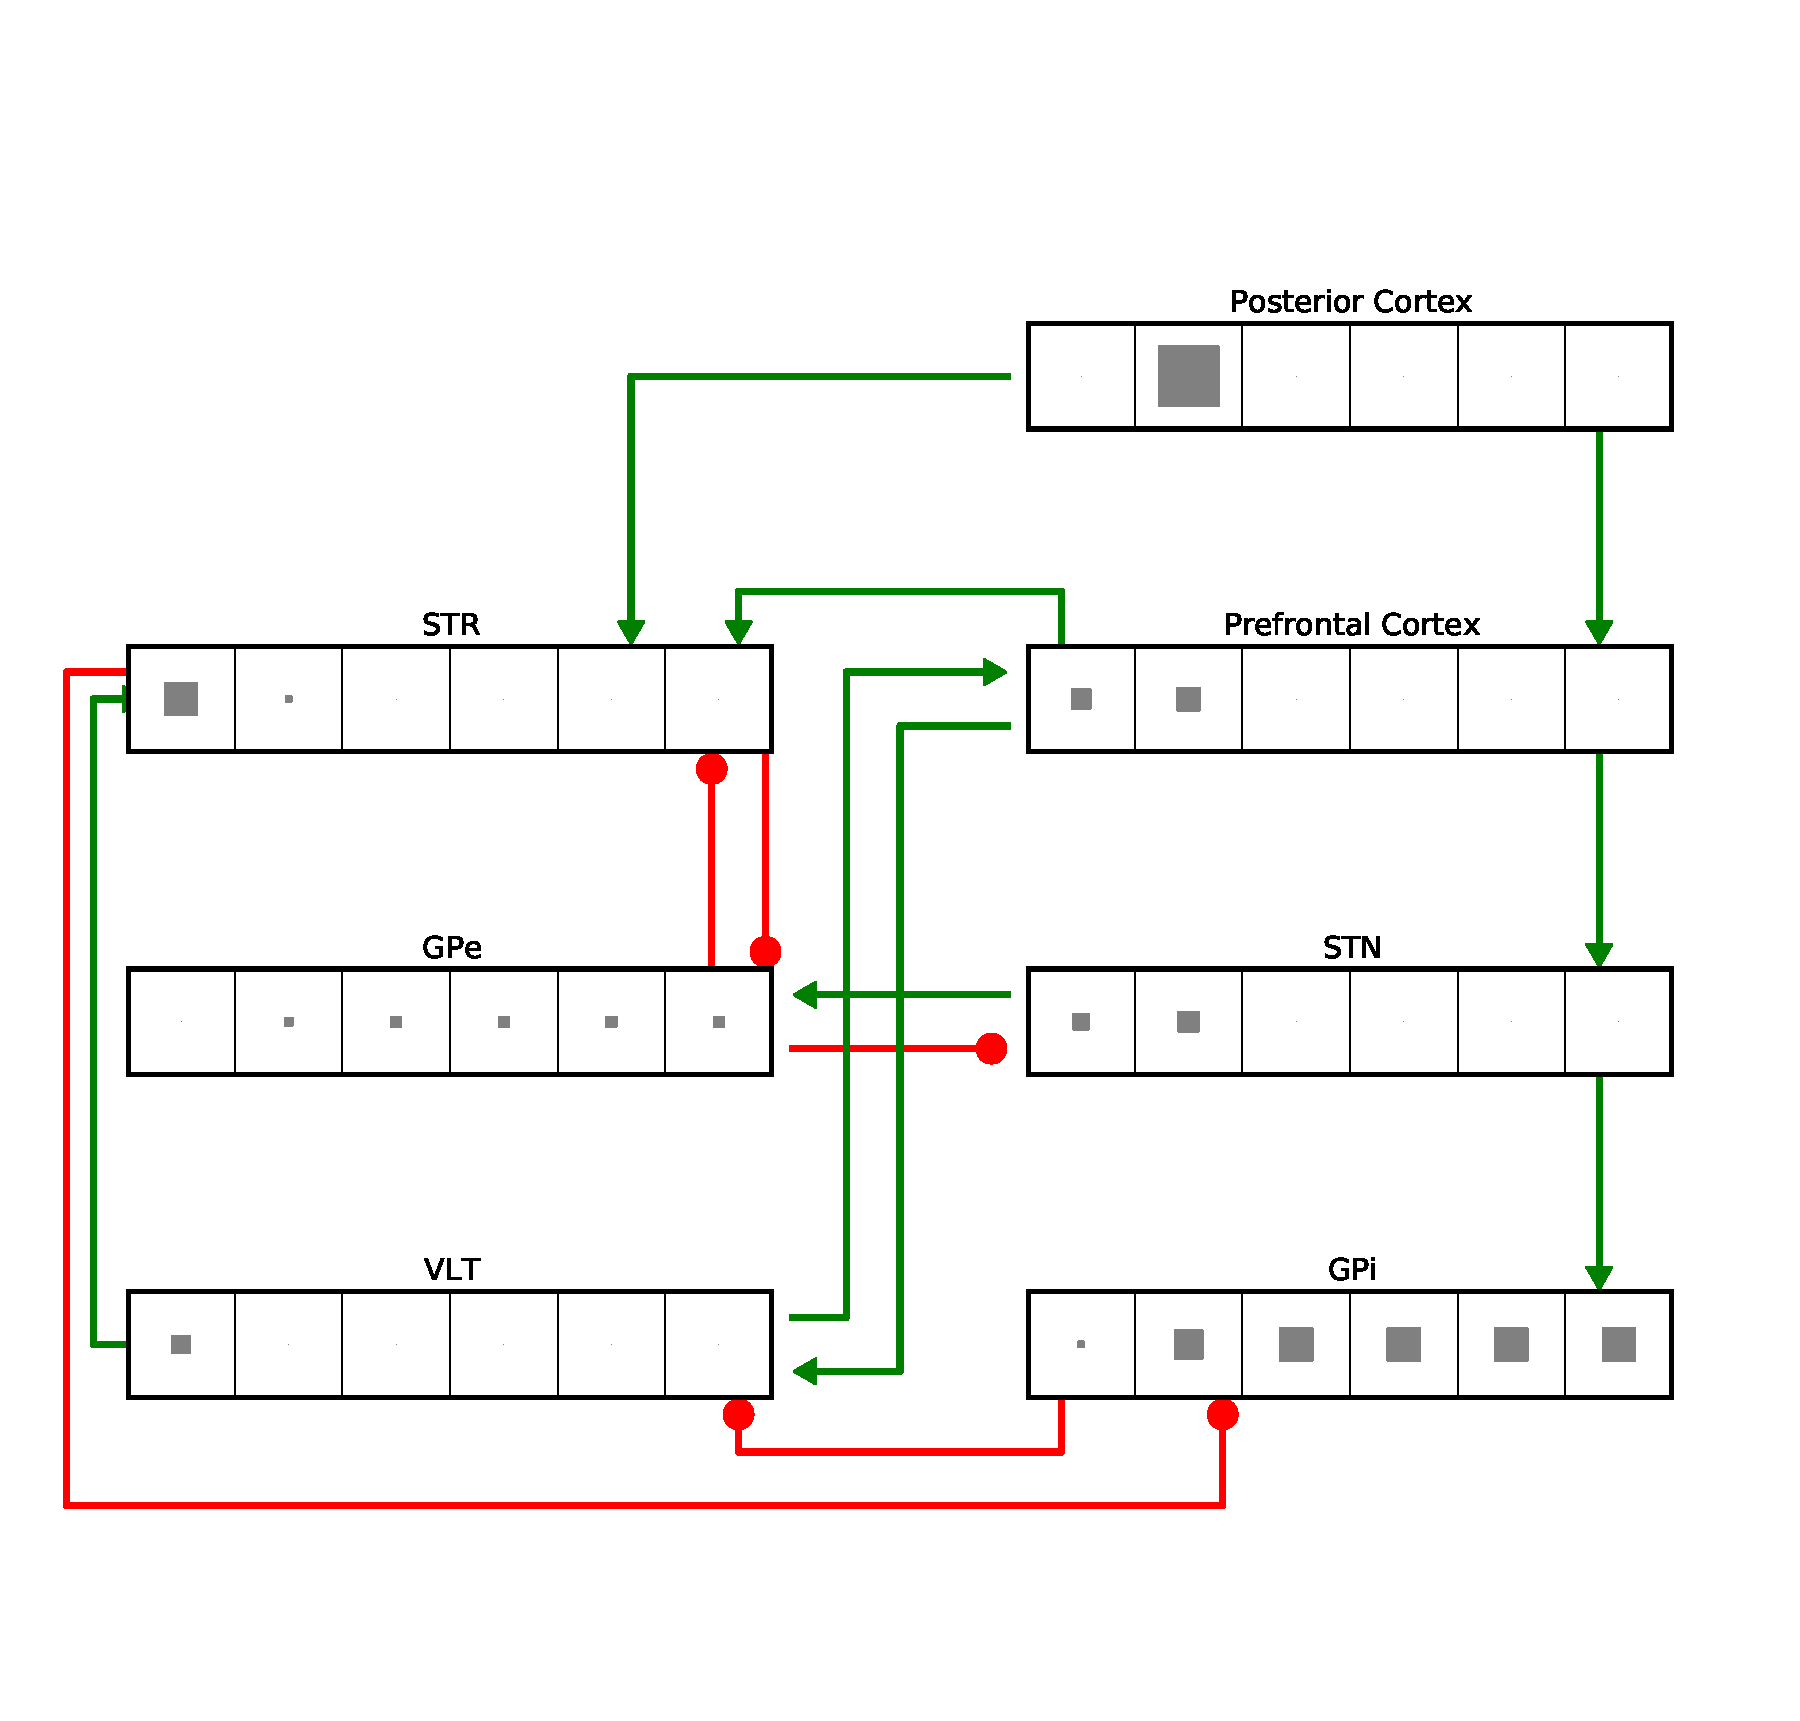
\includegraphics[width=0.4\textwidth]{figures/ch4_11_TBG_1}\\
\hline
t=1.50s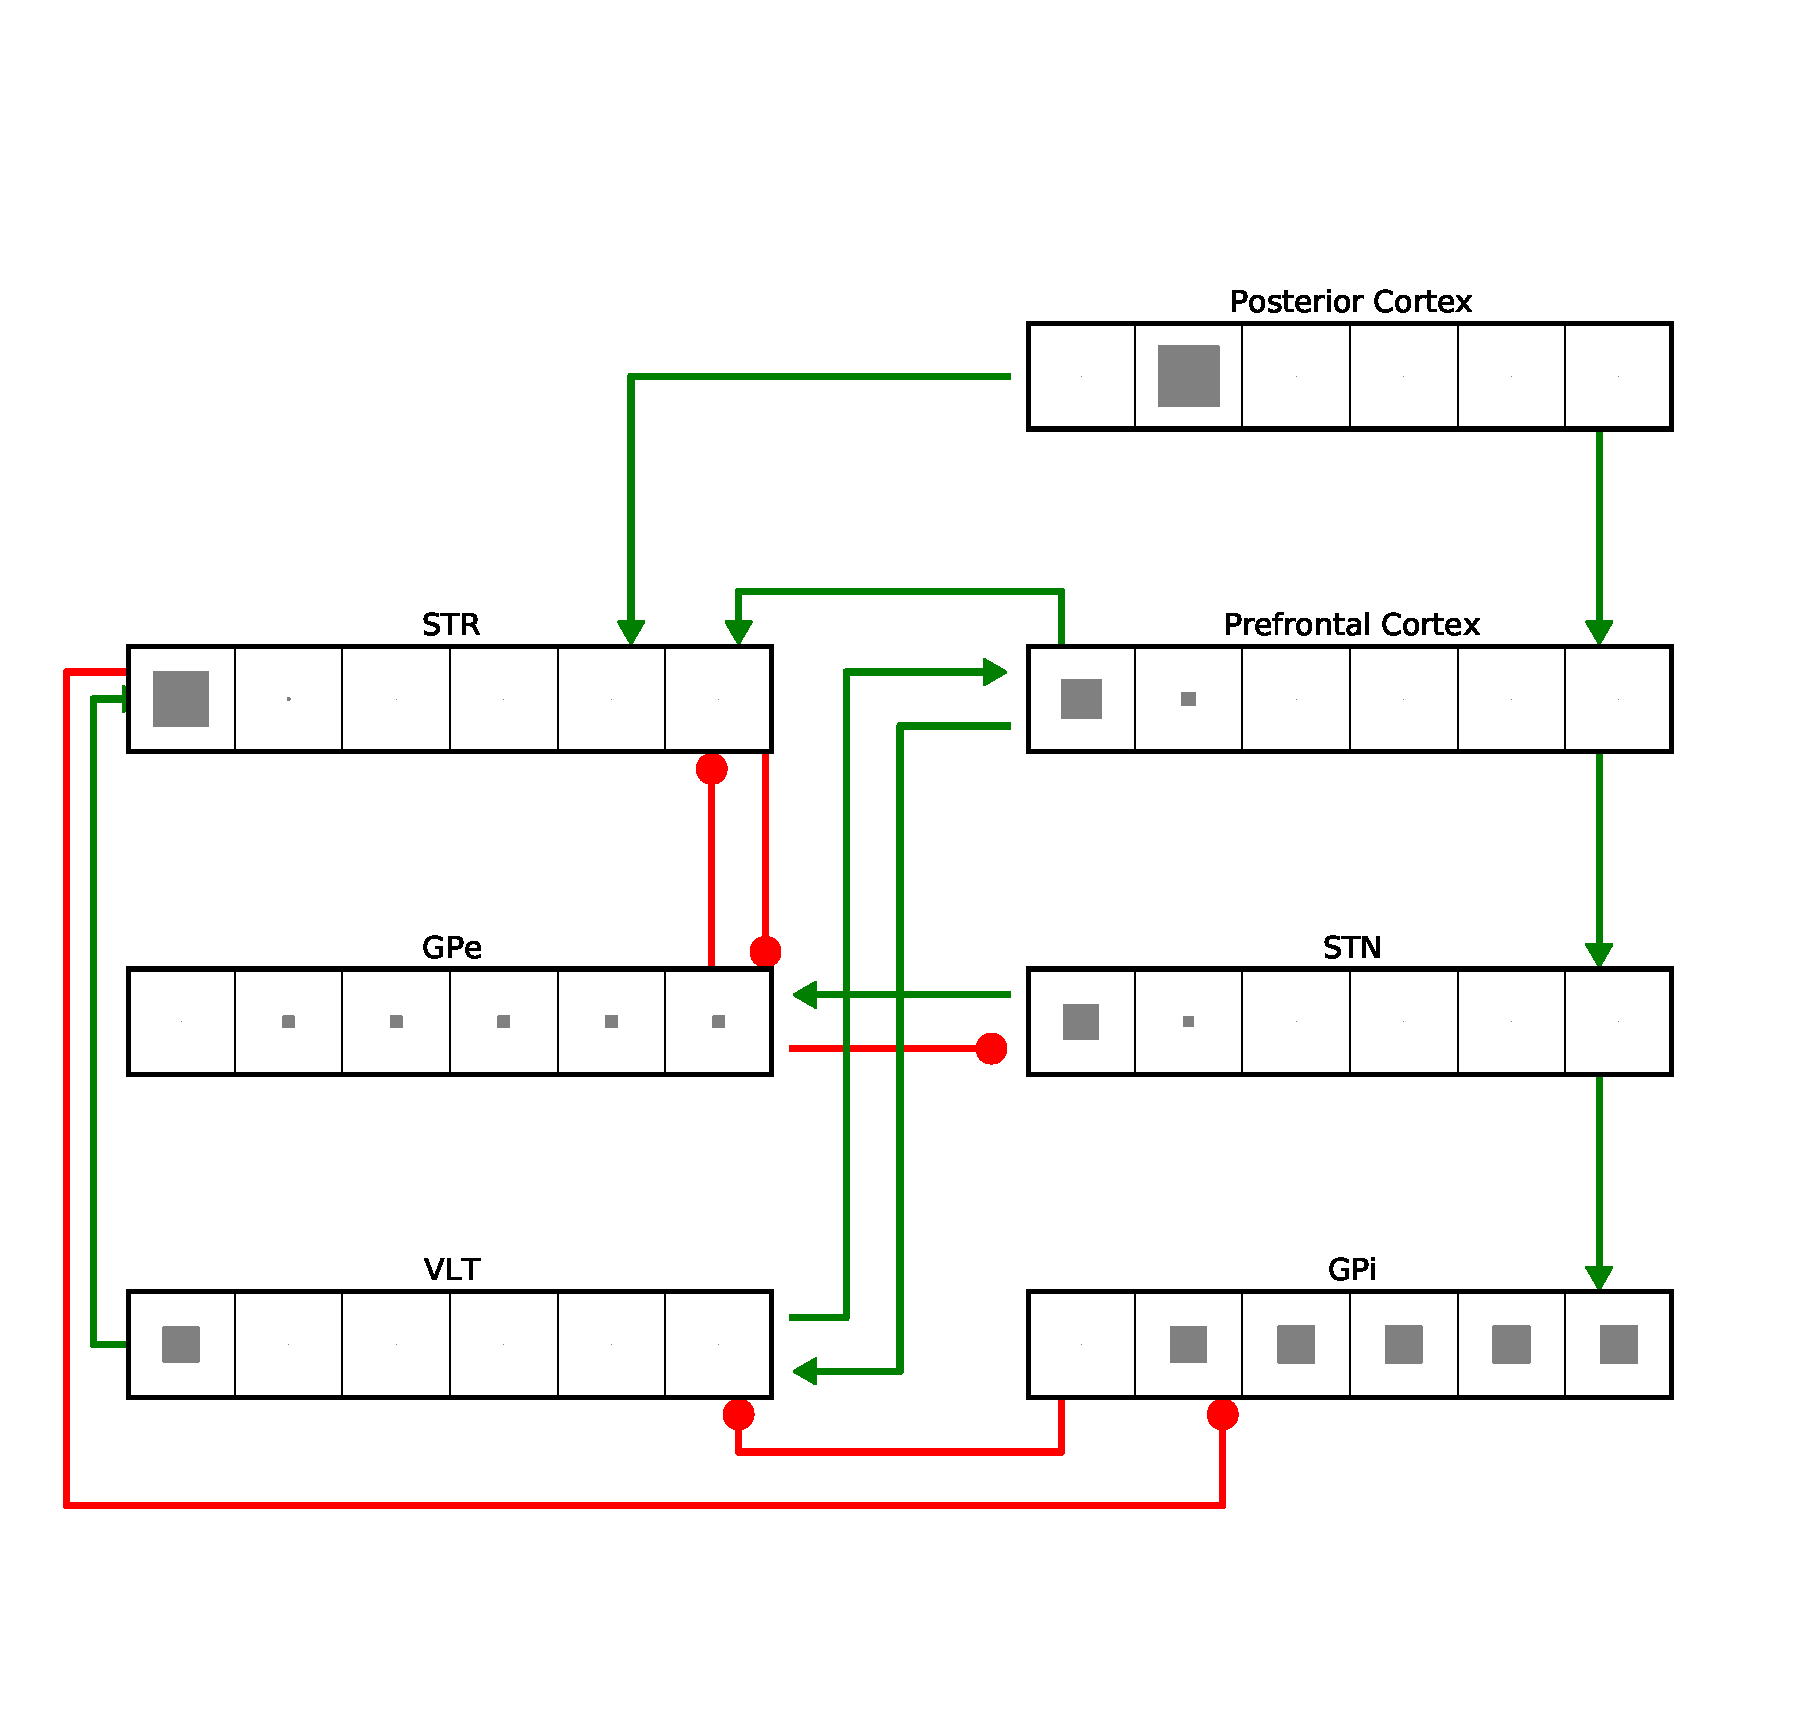
\includegraphics[width=0.4\textwidth]{figures/ch4_11_TBG_15} &
t=2.00s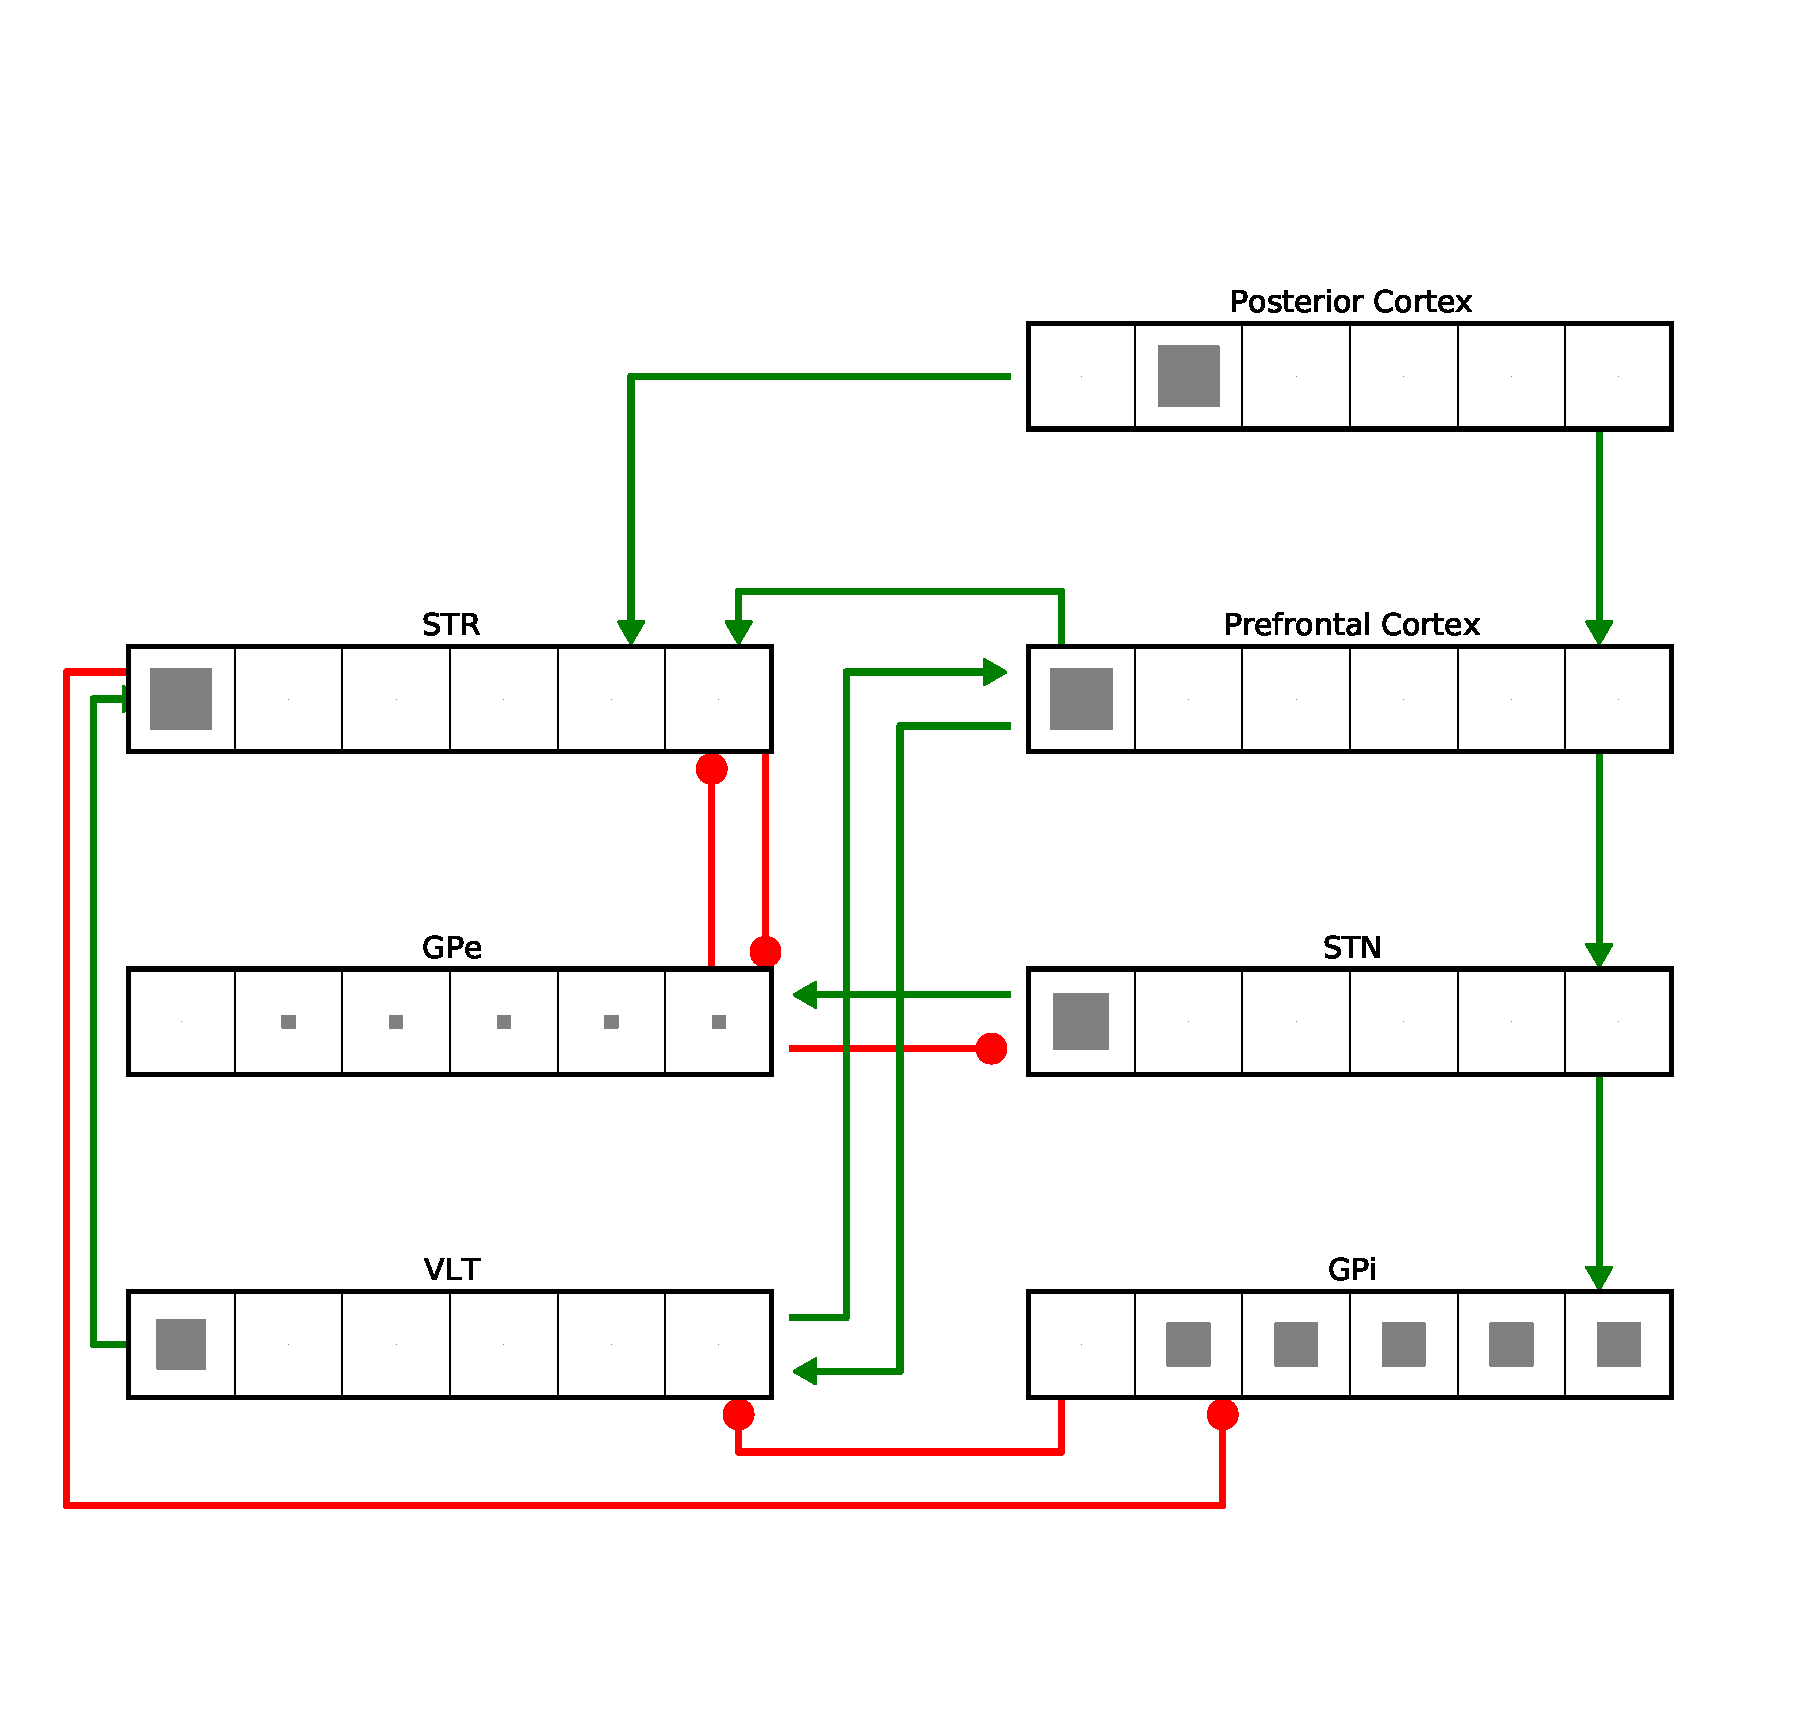
\includegraphics[width=0.4\textwidth]{figures/ch4_11_TBG_2}\\
\hline
\end {tabular}
\caption{ Illustration de sélection de l'action la moins préactivée au niveau de \protect\gls{pfc}. Les carrés pleins représentent les niveaux d'activation aux dates précisées (0.7s,1s,1.5s,2s) durant la simulation. }
\label{Select}

\end{figure}

C'est ainsi qu'on propose le scénario suivant du déroulement de la sélection:
\begin {enumerate}
\item Une cellule est activée dans le \gls{ppc} résultant de l'intégration d'un ensemble d'entrées sensorielles indiquant ainsi qu'une action volontaire est attendue.
\item Le striatum se préactive globalement grâce à la projection totale (tout vers tout) du \gls{ppc} et les cellules correspondant aux actions candidates s'activent au niveau du \gls{pfc} selon les poids des projections \gls{ppc}-\gls{pfc}. Ils s'agit donc de pré-activer les actions que le sujet a l'habitude de faire dans le cadre sensoriel donné.
\item Les \gls{bg} sont donc amenés à sélectionner et présenter au cortex moteur la bonne action à faire et le résultat de l'intégration est servi au cortex frontal moteur et retourné en feedback vers le \gls{str} en passant dans les deux cas par le thalamus.
\item L'inhibition latérale au niveau du cortex peut permettre à elle seule de faire gagner une action mais ne peut pas l'activer vu que la thalamus est en inhibition tonique sous l'effet du \gls{gpi}.  
\item L'activation rapide du \gls{stn} par le \gls{pfc} (par rapport à celle du \gls{str}) implique une excitation diffuse du \gls{gpi} et donc inhibe encore plus les générateurs moteurs de toutes les actions concurrentes permettant ainsi d'arrêter des processus en cours et de faire taire tout les  neurones pour préparer une sélection via un effet on-center/off-surround. 
\item Le striatum fortement bruité commence à faire le basculement grâce à la boucle d'inhibition récurrente avec le \gls{gpe} en étant plus influencé par le feedback du thalamus que par l'entrée du \gls{pfc} et selon le bruit et la différence de saillance une action ou une autre peut gagner la compétition au niveau du \gls{str} et il en sera de même au fur et à mesure dans le \gls{gpi} et Thalamus (chemin direct).
\item Le poids de la connexion \gls{vlt}-\gls{pfc} étant plus fort que le poids réciproque, le thalamus permet de faire basculer l'ordre d'importances des activations au niveau du \gls{pfc} et une action qui est au départ faiblement probable peut gagner la compétition.
\item Le \gls{gpe} permet de stabiliser l'activation du \gls{stn} et d'affaiblir son excitation du \gls{gpi}, mais cette inhibition tonique  \gls{gpe}-\gls{stn} est levée partiellement peu à peu par le \gls{str} permettant ainsi de renforcer d'une part l'effet off-surround  mais peut aussi préparer la récupération de l'activation au niveau du \gls{gpi} si l'excitation qui vient du \gls{stn} devient plus forte que l'inhibition apportée par le \gls{str}.
\end {enumerate}

Nous obtenons donc un mécanisme de sélection actif, permettant d'explorer l'espace d'actions possibles en sélectionnant différents canaux et pouvant donc être complété par un mécanisme d'apprentissage. C'est ce que nous traiterons dans la suite.

\subsubsection{Scénario avec apprentissage}

Nous avons défini une structure (S) composée de structures bi-stables (les unités peuvent prendre seulement deux états 0 ou 1 ) avec des projections tout-vers-tout sur le striatum qui servira pour la représentation d'un contexte motivationnel supplémentaire. L'emplacement de cette struture est discuté dans la suite. Après apprentissage, certaines cellules de cette structure seront recrutées (après plusieurs itérations et par apprentissage comme expliqué dans la suite) pour coder les contextes qui ont été appris. Supposons que l'on est dans un contexte A, l'agent (le modèle) n'a pas cette entrée et tout ce qu'il reçoit comme information sur le contexte est une récompense positive si une action x est choisie et une récompense négative sinon. Cette action n'est pas forcément l'action la plus pré-activée dans le \gls{pfc}.\\

Une épisode d'apprentissage s'étale sur 300 itérations. Une itération dure 4 secondes (2s de computation et 2s de repos). Au début de l'épisode d'apprentissage, une cellule est choisie au hasard et activée dans S. Si la récompense $r$ est positive à la fin de chaque simulation cette cellule est maintenue active et le poids entre elle et la cellule de l'action choisie est renforcé sinon elle est désactivée et une autre cellule de S est activée pour l'itération suivante et le poids est affaibli. Ils s'agit d'un apprentissage hebbien modulé par la récompense selon la règle suivante de mise à jour des poids reliant S au \gls{str} :
 
\begin{center}
\begin{equation} 
W_{S-\gls{str}}= W_{S-\gls{str}}+r*Out_{\gls{str}}*Out_{S}
 \end{equation}
\end{center}

A la fin de l'épisode le système converge vers une cellule maintenue activée et sera étiquetée contexte A. Le poids entre cette cellule et le canal correspondant à l'action x est visiblement renforcé sachant qu'au départ de l'apprentissage on prend une matrice uniforme de poids faibles ($Ws_{S-\gls{str}}=0.01*I$).\\

La matrice de poids suivante est obtenue dans un premier contexte A favorisant le canal 1 après 300 itérations:
\begin{center}
$\begin{pmatrix}
 0.05   &    0.36363874  &    0.01    &    0.04    &    0.02    &     0.02      \\
-0.05   &   -0.07        &    0.01    &   -0.07    &   -0.03    &    -0.05      \\
 0.01   &    0.01        &    0.01    &    0.01    &    0.01    &     0.01     \\
 0.01   &    0.01        &    0.01    &    0.01    &    0.01    &     0.01 \\
 0.01   &    0.01        &    0.01    &    0.01    &    0.01    &     0.01 \\
 0.01   &    0.01        &    0.01    &    0.01    &    0.01    &     0.01 \\
\end{pmatrix}$
\end{center} 
Le poids visiblement renforcé est celui entre la cellule 2 de la structure S et le premier canal des \gls{bg} ($~0.37$), donc il suffit d'activer cette cellule sachant le contexte A pour avoir la sélection souhaitée. Le modèle supporte aussi un sur-apprentissage. En effet, changer vers un contexte B lors de l'apprentissage pendant encore 300 itérations permet d'apprendre une nouvelle correspondance comme le montre la matrice suivante:

\begin{center} 
$\begin{pmatrix}
 0.05   &    0.46929038  &    0.01    &    0.04    &   -0.04    &    -0.02   \\   
-0.05   &   -0.07        &    0.63    &   -0.07    &    0.02    &    -0.03     \\ 
 0.01   &    0.01        &    0.01    &    0.01    &    0.01    &     0.01     \\
 0.01   &    0.01        &    0.01    &    0.01    &    0.01    &     0.01 \\
 0.01   &    0.01        &    0.01    &    0.01    &    0.01    &     0.01 \\
 0.01   &    0.01        &    0.01    &    0.01    &    0.01    &     0.01 \\
\end{pmatrix}$
\end{center} 

Ainsi une autre unité de S est recrutée pour coder le contexte B favorisant un autre canal, le canal 2. Le poids est renforcé (0.63) et en plus le premier apprentissage est sauvegardé. Le durée d'apprentissage d'un contexte (nombre d'itérations minimal dans un épisode) dépend de l'écart entre les saillances des actions candidates, le bruit et l'ordre de changement des contextes.\\

Pour cet apprentissage dépendant du contexte, nous supposons l'existence d'un apprentissage hebbien lent des poids (modification faible des poids entre le \gls{ppc} et le \gls{pfc} par rapport à celle des poids entre S et le \gls{str}) entre le \gls{ppc} et le \gls{pfc} présent en permanence. Le principe est de renforcer les poids entre les cellules des deux structures qui s'activent simultanément. Ainsi la valeur de la pré-activation d'un canal au niveau du \gls{pfc}, correspondant à une activation particulière du \gls{ppc}, est proportionnelle au nombre de fois o\`u l'agent a été amené à choisir l'action correspondant à ce canal dans le même contexte. En d'autres termes, la pré-activation dans le \gls{pfc} reflète ce que l'agent a l'habitude de choisir.
 
\section{Discussion}

Notre modèle, tout comme celui de \gls{gpr} et \gls{cbg}, conserve le mécanisme basique de sélection par désinhibition. Le \gls{str} permet de focaliser la sélection sur l'action la plus importante et le noyau sous-thalamique agit en accord avec le \gls{gpe} via l'excitation diffuse afin de limiter l'activation des unités responsables des canaux à ne pas sélectionner. Le profil d'activité de la réponse du \gls{gpi} présentant trois phases donne un éclaircissement sur la coordination entre les différentes voies au sein des noyaux gris centraux. La première phase de sur-activation de toutes les unités pallidales correspond à l'excitation diffuse par le \gls{stn} via la voie hyperdirecte. Il s'agit d'une phase de préparation à la sélection en renforçant l'inhibition tonique sur le \gls{vlt}, donc s'il y avait un résidu d'activation au niveau de thalamus qui peut altérer la sélection, il sera neutralisé. La deuxième phase correspond au choix sélectif assuré forcément par la voie directe puisque c'est la seule voie inhibant le \gls{gpi}. Les boucles récurrentes assurent la compétition au niveau du \gls{str} pour aboutir à un choix de canal de sélection. Ce choix est traduit au niveau du \gls{gpi} par une baisse de son activation. C'est ainsi que le canal correspondant dans le thalamus est désinhibé et l'action assurée par celui-ci est libérée. La dernière phase est une phase de remise à zero (reset). La sur-activation permet de mettre fin à l'action en cours et vu qu'elle est plus visible au niveau du canal choisi, elle devrait correspondre à la voie indirecte passant par le \gls{str} et le \gls{gpe} assurant aussi le contrôle de la voie hyperdirecte puisqu'elle passe par le \gls{stn}.\\

Une différence principale par rapport à \cite{Gurney:2001a, Girard:2008} est que la saillance des actions n'est pas donnée en amont. Nous proposons un mécanisme d'évaluation de la saillance qui donne plus de liberté dans la détermination de choix de l'action. C'est ainsi que nous attribuons aux \gls{bg} (en particulier au \gls{str}) un rôle plus actif dans la sélection de l'action et qui ne réduit pas la boucle Cortex-\gls{bg}-Thalamus-Cortex à un mécanisme de ``Winner-takes-all''. La saillance des actions candidates est calculée dynamiquement au niveau du \gls{str} sur la base de la réception sensorielle (projection du \gls{ppc}), de l'expérience et des habitudes (projection du \gls{pfc}) et de la motivation ou à un contexte supplémentaire (projection de S). La sélection est donc moins dépendante du classement préalable des actions qui est dans notre cas présent considéré comme une composante parmi d'autres (pré-activation du \gls{pfc}) et l'action gagnante n'est pas déterminée à l'avance. Nous qualifions donc la sélection d'\textit{active}, puisque la saillance est évaluée indirectement et dynamiquement avec une possibilité d'exploration des actions candidates. \\

En effet, le \gls{str} reçoit plusieurs afférences : une entrée corticale non statique influencée par une inhibition latérale (\gls{pfc}), un retour positif du thalamus (\gls{vlt}), une inhibition réciproque du \gls{gpe} et un retour extérieur sous forme de récompense permettant la création d'une mémoire contextuelle (structure S). Les différentes voies internes des \gls{bg} (voie directe, indirecte et hyperdirecte) assurent la sélection au niveau du \gls{gpi} et donc la désinhibition du \gls{vlt}. Puis, le cablage entre les boucles internes des \gls{bg} et la boucle thalamo-corticale permet de mettre en compétition le choix striatal influencé par le bruit et la motivation d'une part et le choix cortical influencé par l'habitude et l'inhibition latérale d'autre part. C'est cette compétition qui permet la sélection d'une action dont la valeur initiale apprise au niveau du \gls{pfc} est faible (fig\ref{Select}). Donc on peut parler de sélection \textit{motivée}.\\

Dans le but d'explorer la possibilité de l'implication des \gls{bg} dans la motivation et le codage de contexte, nous avons proposé un mécanisme d'apprentissage de contexte. L'information sur le contexte n'est pas donné explicitement mais elle est interprétée à travers la récompense. Plusieurs données neurobiologiques confirment que le \gls{str} reçoit un signal dopaminergique global qui peut être interprété comme une fonction de récompense et le fait d'avoir une sélection nette à ce niveau a permis d'expliciter un apprentissage hebbien modulé par la récompense sans avoir besoin d'aller chercher l'action résultante au niveau du \gls{gpi}. En outre, les informations sur les habitudes (l'utilité des actions en dehors du contexte) ne sont pas modifiées, elles restent dans la mémoire de travail assurée par la projection \gls{ppc}-\gls{pfc}.\\

Enfin, la structure S utilisée pour coder le contexte peut correspondre à une partie du \gls{str} différente de celle codant les actions motrices. Il a été reporté dans \cite{Hikosaka:1989, Kimura:2003} qu'il y a des signaux qui dépendent du changement du contexte au niveau de \gls{str}. Des aires corticales de plus haut niveau que le cortex moteur peuvent aussi servir la même fonction. Plus généralement, ce codage de contexte peut être interprété comme la création de représentations de meta-actions que ce soit dans le striatum ou le cortex. Ces m\'eta-actions peuvent à leur tour faire partie d'une boucle Cortex-\gls{bg}-Thalamus-Cortex qui sera coordonnée avec la boucle motrice ce qui rejoint la théorie de la spirale d'Haber \cite{Haber:2000}.\\ 

\cite{Haber:2003} propose une organisation qui s'oppose au postulat de la séparation des circuits moteur, cognitif et limbique incluant les \gls{bg}. Les auteurs proposent une interaction étroite entre ces trois grandes voies. Si le but final d'un traitement de l'information est l'exécution d'une action, l'accomplissement du but recherché nécessite l'activation des processus qui conduisent à cette exécution. D'abord il faut passer par les émotions et la motivation qui initient les comportements. Ensuite, il faut intégrer les fonctions cognitives (ou exécutives) qui organisent et planifient la stratégie de l'exécution de l'action.\\

Ces trois processus sont assurés par les trois grands circuits parallèles décrits précédemment. Considérer que les \gls{bg} sont capables de participer à la création de nouveaux programmes moteurs implique forcément que l'information migre progressivement du compartiment limbique vers le compartiment moteur final via le compartiment cognitif. Chaque composante de l'information serait renvoyée vers son circuit d'origine (la sortie est renvoyée vers la partie corticale stimulée dans le circuit concerné) mais également transférée au circuit suivant. Les processus de prise de décision seraient ainsi influencés par les signaux limbiques puis cognitifs, permettant à l'organisme de s'adapter de manière appropriée à son environnement.\\
